% draft9.tex -- the RETRACTED version (2026-08-08): intro-v2, claim-titles per
% the TOC-alone principle, five figures relocated to Supplement 3, coherence-
% audit fixes applied, closure-measurement limits and reproducibility scoping
% added. draft8.tex is unchanged and remains the target of
% coherence-annotations.edn offsets. Part III here is part3-exotype-v9.tex.
\documentclass[man,12pt,floatsintext,donotrepeattitle]{apa7}

\usepackage{latexml}  % \iflatexml: true under LaTeXML/oxide, false under pdflatex
\usepackage[american]{babel}
\usepackage{csquotes}
\usepackage{amsmath,amssymb}
\usepackage{amsthm}
\usepackage{booktabs}
\usepackage{graphicx}
\usepackage{xcolor}
\usepackage{subcaption}
\usepackage[most]{tcolorbox}
\usetikzlibrary{positioning, arrows.meta, fit, calc, decorations.pathreplacing}
\usepackage{needspace}
\usepackage[style=apa,backend=biber]{biblatex}
\addbibresource{refs.bib}
\usepackage{nameref}
\hypersetup{
  hidelinks,
  pdftitle={Rule-Rewriting Cellular Automata and the Edge of Chaos},
  pdfauthor={Joseph Corneli},
  pdfsubject={Permutation-propagators in cellular automata},
  pdfkeywords={cellular automata, rule evolution, Langton's lambda,
    self-modifying systems, edge of chaos, artificial life, permutation
    operators, exhaustive classification, domain walls}
}

\newcommand{\sig}{\sigma}
\newcommand{\bit}[1]{\mathrm{bit}[#1]}
% Sections are unnumbered in apa7 `man' mode, so \ref{sec:..} is empty;
% cross-reference sections by name instead.
\newcommand{\secref}[1]{\emph{\nameref{#1}}}
% The typed boxes below are tcolorboxes, i.e. TikZ drawings. A converter turns
% TikZ into SVG, which would make most of this document a fixed-geometry
% picture instead of text. Under a converter, define the same environments as
% semantic theorem-like blocks instead. See html-boxes.tex.
% NB: \newif must sit OUTSIDE the guard. When \iflatexml is true TeX skips the
% \else branch by counting \if tokens, and \newif\ifpaperboxfold presents an
% \ifpaperboxfold with no matching \fi, which throws the count off.
\newif\ifpaperboxfold
\iflatexml
  % html-boxes.tex -- converter-side definitions of the paper's typed boxes.
%
% WHY: the print versions of these boxes are tcolorboxes, which are drawn with
% TikZ. latexml-oxide converts TikZ faithfully -- by rendering it as SVG. That
% turns 94% of Supplement 1 and 72% of Supplement 2 into fixed-geometry
% pictures: they do not reflow, they do not scale to a narrow screen, and the
% text inside them is not HTML.
%
% So under a converter we skip tcolorbox entirely and define the same
% environments as ordinary theorem-like blocks. LaTeXML and oxide both emit
% these as <div class="ltx_theorem ltx_theorem_NAME"> with a real title, a real
% counter and a real anchor -- semantic HTML that reflows and can be styled.
%
% Input this from inside an \iflatexml branch, then declare the boxes the
% document actually uses:
%
%     \iflatexml
%       % html-boxes.tex -- converter-side definitions of the paper's typed boxes.
%
% WHY: the print versions of these boxes are tcolorboxes, which are drawn with
% TikZ. latexml-oxide converts TikZ faithfully -- by rendering it as SVG. That
% turns 94% of Supplement 1 and 72% of Supplement 2 into fixed-geometry
% pictures: they do not reflow, they do not scale to a narrow screen, and the
% text inside them is not HTML.
%
% So under a converter we skip tcolorbox entirely and define the same
% environments as ordinary theorem-like blocks. LaTeXML and oxide both emit
% these as <div class="ltx_theorem ltx_theorem_NAME"> with a real title, a real
% counter and a real anchor -- semantic HTML that reflows and can be styled.
%
% Input this from inside an \iflatexml branch, then declare the boxes the
% document actually uses:
%
%     \iflatexml
%       % html-boxes.tex -- converter-side definitions of the paper's typed boxes.
%
% WHY: the print versions of these boxes are tcolorboxes, which are drawn with
% TikZ. latexml-oxide converts TikZ faithfully -- by rendering it as SVG. That
% turns 94% of Supplement 1 and 72% of Supplement 2 into fixed-geometry
% pictures: they do not reflow, they do not scale to a narrow screen, and the
% text inside them is not HTML.
%
% So under a converter we skip tcolorbox entirely and define the same
% environments as ordinary theorem-like blocks. LaTeXML and oxide both emit
% these as <div class="ltx_theorem ltx_theorem_NAME"> with a real title, a real
% counter and a real anchor -- semantic HTML that reflows and can be styled.
%
% Input this from inside an \iflatexml branch, then declare the boxes the
% document actually uses:
%
%     \iflatexml
%       \input{html-boxes}
%       \NewHTMLBox{definition}{Definition}{1}   % 1 = takes a {title} argument
%       \NewHTMLBox{theorem}{Theorem}{0}         % 0 = no title argument
%     \else
%       ... the tcolorbox definitions ...
%     \fi
%
% The [label={...}] option each box carries in the sources is honoured, so
% \ref and \autoref into the boxes keep working.

\usepackage{amsthm}
\usepackage{keyval}

% This file is \input, not a package, so `@` is not a letter here: everything
% touching \define@key or \@empty must sit inside \makeatletter.
\makeatletter

% Option keys. Only `label` does anything; the rest are print-layout keys that
% appear in the sources (fold, breakable=false) and must be absorbed silently.
\define@key{htmlbox}{label}{\def\htmlboxlabel{#1}}
\define@key{htmlbox}{fold}[]{}
\define@key{htmlbox}{unfold}[]{}
\define@key{htmlbox}{breakable}[]{}

\newcommand{\htmlboxsetup}[1]{%
  \def\htmlboxlabel{}%
  \def\htmlbox@opts{#1}%
  \ifx\htmlbox@opts\@empty\else\setkeys{htmlbox}{#1}\fi
  \ifx\htmlboxlabel\@empty\else\expandafter\label\expandafter{\htmlboxlabel}\fi}
\makeatother

% \NewHTMLBox{envname}{Heading}{1 if it takes a mandatory {title}, else 0}
\newcommand{\NewHTMLBox}[3]{%
  % amsthm's default `plain' style italicises the body, which is wrong for
  % findings and worked examples that are pages of prose. `definition' style
  % keeps the body upright and only bolds the heading.
  \theoremstyle{definition}%
  \newtheorem{htmlbox#1}{#2}%
  \ifnum#3=1\relax
    \NewDocumentEnvironment{#1}{O{} m}%
      {\begin{htmlbox#1}[##2]\htmlboxsetup{##1}}%
      {\end{htmlbox#1}}%
  \else
    \NewDocumentEnvironment{#1}{O{}}%
      {\begin{htmlbox#1}\htmlboxsetup{##1}}%
      {\end{htmlbox#1}}%
  \fi}

% Present in the print branch; harmless no-ops here so stray uses do not break.
\providecommand{\foldmark}{}
\providecommand{\thetcbcounter}{}
\makeatletter
\@ifundefined{ifpaperboxfold}{\newif\ifpaperboxfold}{}
\makeatother
\endinput

%       \NewHTMLBox{definition}{Definition}{1}   % 1 = takes a {title} argument
%       \NewHTMLBox{theorem}{Theorem}{0}         % 0 = no title argument
%     \else
%       ... the tcolorbox definitions ...
%     \fi
%
% The [label={...}] option each box carries in the sources is honoured, so
% \ref and \autoref into the boxes keep working.

\usepackage{amsthm}
\usepackage{keyval}

% This file is \input, not a package, so `@` is not a letter here: everything
% touching \define@key or \@empty must sit inside \makeatletter.
\makeatletter

% Option keys. Only `label` does anything; the rest are print-layout keys that
% appear in the sources (fold, breakable=false) and must be absorbed silently.
\define@key{htmlbox}{label}{\def\htmlboxlabel{#1}}
\define@key{htmlbox}{fold}[]{}
\define@key{htmlbox}{unfold}[]{}
\define@key{htmlbox}{breakable}[]{}

\newcommand{\htmlboxsetup}[1]{%
  \def\htmlboxlabel{}%
  \def\htmlbox@opts{#1}%
  \ifx\htmlbox@opts\@empty\else\setkeys{htmlbox}{#1}\fi
  \ifx\htmlboxlabel\@empty\else\expandafter\label\expandafter{\htmlboxlabel}\fi}
\makeatother

% \NewHTMLBox{envname}{Heading}{1 if it takes a mandatory {title}, else 0}
\newcommand{\NewHTMLBox}[3]{%
  % amsthm's default `plain' style italicises the body, which is wrong for
  % findings and worked examples that are pages of prose. `definition' style
  % keeps the body upright and only bolds the heading.
  \theoremstyle{definition}%
  \newtheorem{htmlbox#1}{#2}%
  \ifnum#3=1\relax
    \NewDocumentEnvironment{#1}{O{} m}%
      {\begin{htmlbox#1}[##2]\htmlboxsetup{##1}}%
      {\end{htmlbox#1}}%
  \else
    \NewDocumentEnvironment{#1}{O{}}%
      {\begin{htmlbox#1}\htmlboxsetup{##1}}%
      {\end{htmlbox#1}}%
  \fi}

% Present in the print branch; harmless no-ops here so stray uses do not break.
\providecommand{\foldmark}{}
\providecommand{\thetcbcounter}{}
\makeatletter
\@ifundefined{ifpaperboxfold}{\newif\ifpaperboxfold}{}
\makeatother
\endinput

%       \NewHTMLBox{definition}{Definition}{1}   % 1 = takes a {title} argument
%       \NewHTMLBox{theorem}{Theorem}{0}         % 0 = no title argument
%     \else
%       ... the tcolorbox definitions ...
%     \fi
%
% The [label={...}] option each box carries in the sources is honoured, so
% \ref and \autoref into the boxes keep working.

\usepackage{amsthm}
\usepackage{keyval}

% This file is \input, not a package, so `@` is not a letter here: everything
% touching \define@key or \@empty must sit inside \makeatletter.
\makeatletter

% Option keys. Only `label` does anything; the rest are print-layout keys that
% appear in the sources (fold, breakable=false) and must be absorbed silently.
\define@key{htmlbox}{label}{\def\htmlboxlabel{#1}}
\define@key{htmlbox}{fold}[]{}
\define@key{htmlbox}{unfold}[]{}
\define@key{htmlbox}{breakable}[]{}

\newcommand{\htmlboxsetup}[1]{%
  \def\htmlboxlabel{}%
  \def\htmlbox@opts{#1}%
  \ifx\htmlbox@opts\@empty\else\setkeys{htmlbox}{#1}\fi
  \ifx\htmlboxlabel\@empty\else\expandafter\label\expandafter{\htmlboxlabel}\fi}
\makeatother

% \NewHTMLBox{envname}{Heading}{1 if it takes a mandatory {title}, else 0}
\newcommand{\NewHTMLBox}[3]{%
  % amsthm's default `plain' style italicises the body, which is wrong for
  % findings and worked examples that are pages of prose. `definition' style
  % keeps the body upright and only bolds the heading.
  \theoremstyle{definition}%
  \newtheorem{htmlbox#1}{#2}%
  \ifnum#3=1\relax
    \NewDocumentEnvironment{#1}{O{} m}%
      {\begin{htmlbox#1}[##2]\htmlboxsetup{##1}}%
      {\end{htmlbox#1}}%
  \else
    \NewDocumentEnvironment{#1}{O{}}%
      {\begin{htmlbox#1}\htmlboxsetup{##1}}%
      {\end{htmlbox#1}}%
  \fi}

% Present in the print branch; harmless no-ops here so stray uses do not break.
\providecommand{\foldmark}{}
\providecommand{\thetcbcounter}{}
\makeatletter
\@ifundefined{ifpaperboxfold}{\newif\ifpaperboxfold}{}
\makeatother
\endinput

  \NewHTMLBox{workedexample}{Worked example}{1}
  \NewHTMLBox{theorem}{Theorem}{0}
  \NewHTMLBox{definition}{Definition}{1}
  \NewHTMLBox{corollary}{Corollary}{0}
  \NewHTMLBox{proposition}{Proposition}{1}
  \NewHTMLBox{empiricalfinding}{Empirical finding}{1}
  \NewHTMLBox{observation}{Observation}{1}
\else
\tcbset{%
  fold/.code={%
    \paperboxfoldtrue
    \pgfkeysalso{top=0pt,bottom=0pt,boxsep=0pt}},
  unfold/.code={\paperboxfoldfalse}}
\newcommand{\foldmark}{%
  \ifpaperboxfold\space{\normalfont\scriptsize[folded]}\fi}

\newtcolorbox[auto counter]{workedexampleframe}[2][]{%
  enhanced,
  breakable,
  colback=green!6,
  colframe=green!45!black,
  boxrule=0.7pt,
  arc=1.5mm,
  left=2.5mm,
  right=2.5mm,
  top=1.5mm,
  bottom=1.5mm,
  fonttitle=\bfseries,
  title={Worked example~\thetcbcounter: #2\foldmark},
  #1}
\NewDocumentEnvironment{workedexample}{O{} m +b}{%
  \paperboxfoldfalse
  \begin{workedexampleframe}[#1]{#2}%
    \ifpaperboxfold\else#3\fi
  \end{workedexampleframe}}{}

% --- typed boxes for compression -------------------------------------------
% Each typed box accepts `fold` in its option list. Folding preserves its
% counter, title, label, and cross-references while suppressing only the body.
\newtcolorbox[auto counter]{theoremframe}[1][]{%
  enhanced, breakable, colback=blue!5, colframe=blue!55!black,
  boxrule=0.7pt, arc=1.5mm, left=2.5mm, right=2.5mm,
  top=1.5mm, bottom=1.5mm, fonttitle=\bfseries,
  title={Theorem~\thetcbcounter\foldmark}, #1}
\NewDocumentEnvironment{theorem}{O{} +b}{%
  \paperboxfoldfalse
  \begin{theoremframe}[#1]%
    \ifpaperboxfold\else#2\fi
  \end{theoremframe}}{}

\newtcolorbox[auto counter]{definitionframe}[2][]{%
  enhanced, breakable, colback=violet!6, colframe=violet!55!black,
  boxrule=0.7pt, arc=1.5mm, left=2.5mm, right=2.5mm,
  top=1.5mm, bottom=1.5mm, fonttitle=\bfseries,
  title={Definition~\thetcbcounter: #2\foldmark}, #1}
\NewDocumentEnvironment{definition}{O{} m +b}{%
  \paperboxfoldfalse
  \begin{definitionframe}[#1]{#2}%
    \ifpaperboxfold\else#3\fi
  \end{definitionframe}}{}

% Corollaries auto-boxed like theorems (blue). Empirical findings are amber:
% observed (not proved) claims live here, the validated home for rewritten results.
\newtcolorbox[auto counter]{corollaryframe}[1][]{%
  enhanced, breakable, colback=blue!5, colframe=blue!55!black,
  boxrule=0.7pt, arc=1.5mm, left=2.5mm, right=2.5mm,
  top=1.5mm, bottom=1.5mm, fonttitle=\bfseries,
  title={Corollary~\thetcbcounter\foldmark}, #1}
\NewDocumentEnvironment{corollary}{O{} +b}{%
  \paperboxfoldfalse
  \begin{corollaryframe}[#1]%
    \ifpaperboxfold\else#2\fi
  \end{corollaryframe}}{}

\newtcolorbox[auto counter]{propositionframe}[2][]{%
  enhanced, breakable, colback=blue!5, colframe=blue!55!black,
  boxrule=0.7pt, arc=1.5mm, left=2.5mm, right=2.5mm,
  top=1.5mm, bottom=1.5mm, fonttitle=\bfseries,
  title={Proposition~\thetcbcounter: #2\foldmark}, #1}
\NewDocumentEnvironment{proposition}{O{} m +b}{%
  \paperboxfoldfalse
  \begin{propositionframe}[#1]{#2}%
    \ifpaperboxfold\else#3\fi
  \end{propositionframe}}{}

\newtcolorbox[auto counter]{empiricalfindingframe}[2][]{%
  enhanced, breakable, colback=orange!7, colframe=orange!65!black,
  boxrule=0.7pt, arc=1.5mm, left=2.5mm, right=2.5mm, top=1.5mm, bottom=1.5mm,
  fonttitle=\bfseries,
  title={Empirical finding~\thetcbcounter: #2\foldmark}, #1}
\NewDocumentEnvironment{empiricalfinding}{O{} m +b}{%
  \paperboxfoldfalse
  \begin{empiricalfindingframe}[#1]{#2}%
    \ifpaperboxfold\else#3\fi
  \end{empiricalfindingframe}}{}

% Observations (teal): consequences/remarks pulled out of definitions and prose.
\newtcolorbox[auto counter]{observationframe}[2][]{%
  enhanced, breakable, colback=teal!7, colframe=teal!55!black,
  boxrule=0.7pt, arc=1.5mm, left=2.5mm, right=2.5mm, top=1.5mm, bottom=1.5mm,
  fonttitle=\bfseries, title={Observation~\thetcbcounter: #2\foldmark}, #1}
\NewDocumentEnvironment{observation}{O{} m +b}{%
  \paperboxfoldfalse
  \begin{observationframe}[#1]{#2}%
    \ifpaperboxfold\else#3\fi
  \end{observationframe}}{}
\fi

% Supplement pointers. These are not box machinery and must stay outside the
% guard above, or they vanish from the converted build.
% Empirical findings live canonically in the literate notebook submitted as
% Supplement 1. Keep only stable, compact pointers in the narrative.
\newcommand{\suppfindingref}[1]{Supplement~1, Box~#1}
% Formal apparatus lives canonically in Supplement 2. The narrative states each
% result in prose where it is used and points here for statement and proof.
\newcommand{\supptheorytext}[2]{Supplement~2, #1: #2.}
\newcommand{\supptheory}[2]{\footnote{\supptheorytext{#1}{#2}}}
\newcommand{\suppfindingtext}[2]{\suppfindingref{#1}: #2.}
\newcommand{\suppfinding}[2]{\footnote{\suppfindingtext{#1}{#2}}}
% Structured-proof outline commands (Figures 1a-1c).
\newcommand{\ptag}[2]{\textcolor{#1}{\textbf{\scriptsize[#2]}}}
\newcommand{\tagthm}{\ptag{blue!55!black}{thm}}
\newcommand{\tagdef}{\ptag{violet!55!black}{def}}
\newcommand{\tagmeas}{\ptag{orange!75!black}{meas}}
\newcommand{\tagctrl}{\ptag{teal!60!black}{ctrl}}
\newcommand{\tagneg}{\ptag{green!40!black}{neg}}
\newcommand{\tagprobe}{\ptag{purple!70!black}{probe}}
\newcommand{\pstep}[2]{\par\hangindent=11mm\hangafter=1\noindent\makebox[11mm][l]{$\langle#1\rangle$}#2}
\newcommand{\galleryitem}[3][.31\linewidth]{\begin{minipage}[t]{#1}\centering
  \includegraphics[width=\linewidth,height=30mm,keepaspectratio]{#2}\\[1.5pt]
  {\scriptsize #3}\end{minipage}}
% Adjacent supplement pointers merge into one note: footmisc's `multiple' is
% defeated by hyperref, which apa7 loads itself, and one marker reads better.
\newcommand{\suppnote}[1]{\footnote{#1}}

\title{Rule-Rewriting Cellular Automata and the Edge of Chaos}
\shorttitle{Roule-Rewriting Cellular Automata}
\authorsnames{Joseph Corneli}
\authorsaffiliations{{Oxford Brookes University, Oxford OX3 0BP, United Kingdom},
  {Hyperreal Enterprises Ltd, United Kingdom}}
\note{Corresponding author: Joseph Corneli,
  \href{mailto:jcorneli@brookes.ac.uk}{jcorneli@brookes.ac.uk}.}

\abstract{%
We study cellular automata in which each cell carries, alongside its binary state,
the eight-bit rule it executes, and in which operators rewrite those rules as the
system runs. A rule-rewriting operator is defined by a permutation $\sig$ of the eight truth-table
positions: it writes the negation of position $p$ to position $\sig(p)$. The
resulting family of $8! = 40{,}320$ operators is classified exactly, with the
central statements formally verified: an operator has an unchanged rule exactly when
every cycle of $\sig$ has even length; a permutation with $k$ cycles, all even, has
$2^k$ unchanged rules; and every unchanged rule has four of its eight outputs
active, so Langton's activity parameter is $1/2$ at every fixed point. The
classical edge-of-chaos coordinate therefore cannot distinguish these operators, and
in a finite-size scan the transition region does not sharpen with lattice size, so
we find no critical point. We then expand the class of automata architectures, and examine criticality by measuring how far the effect of a single-cell
change travels once a run is forked. In every architecture tested, that distance is
governed by whether rule updates read the current state field: removing the
state-to-rule input roughly halves it; replacing a growing fraction of current state
readings with readings of a frozen copy of matched spatial statistics reduces it
smoothly; and rule diversity, mutation, refuges, niches, and rule mobility leave it
unchanged. A locally triggered gate reproduces the same ordering---reading current
states raises the distance, reading a frozen field of matched statistics and firing
rate lowers it. Finally, we make the operator assignment itself a per-cell heritable
state---an exotype---and ask whether local dynamics alone can find and hold the
regime in which frozen and changing regions coexist and merge into visibly complex patterns.  An external
selection policy helped us find this regime interactively. Within the tested family of exotypes, local selection was not able to recover the observed behaviour.
However, we constructed local interventions that do prevent freezing, and hold a foam of small frozen islands, rather than the exotype-driven configuration's extended complex regions.}  \keywords{cellular automata, rule evolution,
  Langton's lambda, self-modifying systems, edge of chaos, artificial
  life, permutation operators, exhaustive classification, damage
  spreading, perturbation analysis}

% Artificial Life asks for the abstract and keywords on the cover page and the
% main text on page 2. In apa7 manuscript mode, suppress the page break that
% normally separates the title page from the abstract; retain the following
% page break before the main text.
% HTML has no title page, and under a converter \maketitle is the kernel's, so
% these patches cannot match and their \PackageError branches fire spuriously.
% Guarding keeps the tripwire intact for the PDF build.
\iflatexml\else
\makeatletter
\patchcmd{\maketitle}{\vspace*{4\baselineskip}}{\vspace*{\baselineskip}}%
  {}{\PackageError{draft5}{Could not compact title-page spacing}{}}
\patchcmd{\maketitle}{\newpage}{\vspace{0pt}}%
  {}{\PackageError{draft5}{Could not place abstract on title page}{}}
\makeatother
\fi

\begin{document}
\maketitle

\input{intro-v2-generated}

Figures~\ref{fig:map-a}--\ref{fig:map-c} carry that outline in
structured-proof form, one assertion per part. Each step is tagged by
the kind of evidence behind it: theorems verified in Lean~4,
constructions, measurements, matched controls, audited negative
results, and the two probes directed by the related-work
audit. Beneath each outline runs a gallery of details cut from the
evidence itself---spacetime plates and damage fields---each
cross-referenced to the figure that develops it and to the numbered
step it illustrates, so the series can be read as a visual index of
the paper as well as its logical skeleton.  A scope seam runs through
the outline, and it is deliberate. Assertions
$\langle1.1\rangle$--$\langle1.2\rangle$ establish a coordinate;
assertion $\langle1.3\rangle$ concerns a regime. The operator family
is shared between them, but the evidence is not: no step of
$\langle1.3\rangle$ cites a measurement of $\langle1.2\rangle$, and
reach does not predict regime ($R^2 = 0.02$).

\begin{table}[tbp]
\caption{The four kinds of object studied. Each measurement attaches to one
row; no result in this paper transfers between rows.}
\label{tab:objects}
\begin{tabular}{@{}p{0.14\linewidth}p{0.30\linewidth}p{0.44\linewidth}@{}}
\toprule
Where & Object & What is measured on it \\
\midrule
Part~I & Rule-rewriting operators $P_\sig$ (all $40{,}320$) &
fixed rules, their activity, and an exhaustive census of which operators
sustain diverse rule fields \\
Part~II & Fixed update architectures composing operators with a
state-reading step & how far a one-cell perturbation travels, under
ablation of the state-to-rule input and under the graded-staleness dial \\
--- & Conditional compositions (gates) whose firing condition is computed
from the lattice & perturbation travel at matched firing rates: blind,
current-state, and frozen-state conditions \\
Part~III & Exotype lattices, where the operator assignment is itself
per-cell state & phase outcomes under an optimizing selection policy, and
controls with the policy removed \\
\bottomrule
\end{tabular}
\end{table}

\begin{figure}[tbp]
\centering
\begin{minipage}{\linewidth}\small
\setlength{\parskip}{2pt}
\pstep{1.1}{\textbf{Assertion (Part~I).} The classical edge-of-chaos
coordinate cannot govern this family.}
\pstep{1.1.1}{\tagdef\ A rule-rewriting operator is a permutation $\sig$ of the eight
truth-table positions, writing $\neg g(k)$ to position $\sig(k)$; the family
has $8!=40{,}320$ members.}
\pstep{1.1.2}{\tagthm\ An operator leaves some rule unchanged iff every cycle
of $\sig$ is even (Lean~4).}
\pstep{1.1.3}{\tagthm\ An all-even $\sig$ with $k$ cycles fixes exactly $2^k$
rules, and every fixed rule has activity $\lambda=\tfrac12$ (Lean~4).}
\pstep{1.1.4}{\tagmeas\ Census of all cycle types: odd-cycle operators
sustain diverse rule fields; all-even types split---by the specific
permutation, not its cycle type.}
\pstep{1.1.5}{\tagneg\ Finite-size scan: the order--disorder crossover does
not narrow as the lattice grows; no critical point at tested sizes.}
\pstep{1.1.6}{By $\langle1.1.3\rangle$, $\lambda$ is constant where it would
have to discriminate; by $\langle1.1.4\rangle$--$\langle1.1.5\rangle$ neither
cycle algebra nor a parameter scan replaces it. Propagation must be measured
causally $\rightarrow\langle1.2\rangle$.}
\medskip

\noindent\galleryitem[.235\linewidth]{figures/details/d-fig2pair.png}{The
2015 operator collapses its genotype---Fig.~\ref{fig:fig2pair},
$\langle1.1.1\rangle$}\hfill
\galleryitem[.235\linewidth]{figures/details/d-parity.png}{Even cycles:
fixed point exists, field settles---Fig.~\ref{fig:parity},
$\langle1.1.2\rangle$}\hfill
\galleryitem[.235\linewidth]{figures/details/d-shell.png}{Dead genotype,
live phenotype at $\lambda=\frac12$---Fig.~\ref{fig:shell},
$\langle1.1.3\rangle$}\hfill
\galleryitem[.235\linewidth]{figures/details/d-rule110.png}{One operator
concentrates Rule~110---Fig.~\ref{fig:regimes},
$\langle1.1.4\rangle$}
\end{minipage}
\renewcommand{\thefigure}{1a}
\caption{\textbf{Argument outline, I: the classical coordinate dies.}
Structured-proof form; steps tagged \tagthm\ are theorems verified in
Lean~4, \tagdef\ are constructions, and \tagmeas/\tagctrl/\tagneg\ are
empirical---measurements, matched controls, and audited negative results
(\tagprobe, in Figure~1c, marks experiments directed by the related-work
audit). Below the steps, the evidence in miniature: each detail is
cross-referenced to the figure that develops it and to the step it
illustrates.}
\label{fig:map-a}
\addtocounter{figure}{-1}
\end{figure}

\begin{figure}[tbp]
\centering
\begin{minipage}{\linewidth}\small
\setlength{\parskip}{2pt}
\pstep{1.2}{\textbf{Assertion (Part~II).} Whether rule updates read current
cell states governs how far a perturbation reaches; nothing else tested
does.}
\pstep{1.2.1}{\tagdef\ The river: a collapsing propagator composed with a
phenotype-reading construction step, sustaining structured phenotype
indefinitely.}
\pstep{1.2.2}{\tagmeas\ Fork-and-flip causal reach, calibrated on elementary
rules: the river reaches $12.97$ reading live states, $5.51$ with the read
ablated.}
\pstep{1.2.3}{\tagctrl\ A dial replacing live reads with a frozen field of
matched spatial statistics: reach monotone in causal currency, spanning
$1.28$--$12.97$.}
\pstep{1.2.4}{\tagneg\ Sustained diversity, mutation, refuges, niches, and
mobility leave reach unchanged; conservative transport alone also moves it,
breaking the diversity confound.}
\pstep{1.2.5}{\tagmeas\ Independent re-derivation: a local gate that is blind
reproduces the prescribed-rate baseline; reading live states exceeds it;
reading a matched frozen field falls below it, in every tested pair.}
\medskip

\noindent\galleryitem{figures/details/d-river.png}{The river's phenotype
domains, sustained by the read---Fig.~\ref{fig:river},
$\langle1.2.1\rangle$}\hfill
\galleryitem{figures/details/d-cone-river.png}{The measurement: one flip's
damage cone, live edge---Fig.~\ref{fig:regime-placement},
$\langle1.2.2\rangle$}\hfill
\galleryitem{figures/details/d-gate-pair.png}{Live gate spreads damage;
frozen gate does not---Fig.~\ref{fig:frozen-gate},
$\langle1.2.5\rangle$}
\end{minipage}
\renewcommand{\thefigure}{1b}
\caption{\textbf{Argument outline, II: causal currency governs reach.} The
gallery: the river's phenotype, the damage cone that is the measurement, and
the gate pair in which the same one-flip cone spreads under a live read and
collapses to a needle under a frozen one.}
\label{fig:map-b}
\addtocounter{figure}{-1}
\end{figure}

\begin{figure}[tbp]
\centering
\begin{minipage}{\linewidth}\small
\setlength{\parskip}{2pt}
\pstep{1.3}{\textbf{Assertion (Part~III).} The coexistence regime is locally
produced and default-abundant; what is missing is a locally computable
certificate of it, and any tested way back to the found configuration.}
\pstep{1.3.1}{\tagdef\ The exotype: $\sig$ becomes per-cell state,
transmitted between neighbours under a selection rule with precision
$\beta$.}
\pstep{1.3.2}{\tagmeas\ Three outcomes at tested parameters: the changing
phase wins, the frozen phase wins, or both persist for the full horizon (the
found configuration).}
\pstep{1.3.3}{\tagneg\ No tested local quantity ranks operators from within a
run: the field a cell would need decorrelates in ${\sim}6$ steps, inside any
discriminating window.}
\pstep{1.3.4}{\tagctrl\ Adoption switched off: $30/30$ control runs neither
freeze nor die---coexistence is the substrate's default; freezing is the
policy's effect at high $\beta$.}
\pstep{1.3.5}{\tagprobe\ The freeze is nucleation-limited, the bistable
phenomenology co-evolving substrates predict \parencite{gross2006epidemic}:
an established frozen front invades ($5/6$ seeds), yet the frozen phase
never arises from developed churn ($0/6$ in $10^4$ steps)---two macrostates
at matched parameters, selected by history.}
\pstep{1.3.6}{\tagprobe\ A one-sided rule in the design class of
\textcite{droste2013analytical}---write only into long-settled
cells---holds a mixed state at a sixth of the dose of its randomly placed
yoke: placement informs once the trigger is one-sided; the held state is a
foam, not $\langle1.3.2\rangle$'s found configuration.}
\medskip

\noindent\galleryitem{figures/details/d-lavalamp.png}{The found configuration:
structured and chaotic regimes side by side---Fig.~\ref{fig:exo-lavalamp},
$\langle1.3.2\rangle$}\hfill
\galleryitem{figures/details/d-bifurcation.png}{High-precision adoption:
the freeze invades within ${\sim}500$ steps---Fig.~\ref{fig:exo-bifurcation},
$\langle1.3.4\rangle$}\hfill
\galleryitem{figures/details/d-foam.png}{What undirected writes hold: a
foam---Fig.~\ref{fig:interventions}, $\langle1.3.6\rangle$}
\end{minipage}
\renewcommand{\thefigure}{1c}
\caption{\textbf{Argument outline, III: a regime without a certificate.}
The gallery shows the found configuration, the absorbing endpoint that
high-precision adoption produces, and the foam that undirected writes hold
instead.}
\label{fig:map-c}
\renewcommand{\thefigure}{\arabic{figure}}
\end{figure}

\clearpage
\section{Related Work: A New Operator Family Among Familiar Phenomena}
\label{sec:related}

The idea that a cellular automaton's rule can itself be a dynamical variable
is not new. Structurally dynamic CA couple the lattice topology to the value
field while leaving the local function fixed \parencite{ilachinski1987structurally};
rule-changing and self-referential CA let the state field modify the update
\parencite{mori1998rulechanging,pavlic2014selfref}; the Game of Life has been
run under step-by-step rule switching \parencite{miszczak2023ruleswitching};
and graph-rewriting automata embed their own rule set as manipulable data in
the spirit of von Neumann's constructors \parencite{tomita2007selfdescription}.
Per-cell rules are likewise established: cellular programming co-evolves a
rule per cell with neighbour exchange \parencite{sipper1996coevolving}, non-uniform
CA are a standard object \parencite{dennunzio2011nonuniform}, and, closest to our
construction, \textcite{khajehabdollahi2023locally} attach local rule
parameters to each cell of an Ising lattice and update them online from the
state field---the genotype--phenotype split of \secref{sec:object}, two years
earlier and in another community. What none of these supplies is the object
this paper studies: a group-theoretic family of rule-table maps, enumerated
exhaustively, applied as the update law of a running lattice, with the
operator's fixed-point structure derived as a theorem. The nearest formal
neighbours each break at least two of those four conjuncts:
\textcite{cattaneo1997transformations} classify transformations of rule
space exactly, but as static conjugacies applied once, not iterated
operators; \textcite{lipackard1990structure} apply operators to truth-table
positions across all $256$ rules, but their family is the eight single-bit
flips, which have no interesting fixed-point structure where an $S_8$ action
does; and the most recent comprehensive CA taxonomy has five families and no
category for rules rewritten during evolution \parencite{rollier2024taxonomy}.
The symmetry group the ECA literature does use is reflection~$\times$
complement, of order four \parencite{svozil2025symmetries}; it is not $S_8$,
and the negation-carrying family of Equation~\eqref{eq:prop} does not appear
in it.

The balance half of Part~I's theorem has an ancestor that must be named:
Hedlund's theorem that every surjective CA is balanced pins the most
canonical structural subfamily of rule space at $\lambda = 1/2$
\parencite{hedlund1969endomorphisms}, and the constraint-forces-balance
mechanism remains active in general settings \parencite{capobianco2017postsurjectivity},
including non-uniform CA \parencite{paturi2025reversibility}---the setting our
lattice instantaneously is. $\lambda$ is also known to be many-to-one at
mid-range generally \parencite{sakai2002lambdaF}. What Part~I adds is not
that a structural condition forces balance but \emph{where} the degeneracy
lands: on the fixed-point set of a rule-rewriting operator, the set the rule
dynamics itself selects. That a rule-table coordinate underdetermines the
dynamics is meanwhile a recognised open problem
\parencite{vispoel2022classification}, and the edge-of-chaos hypothesis the
coordinate served remains contested in both its biological and its
computational forms
\parencite{teuscher2022revisiting,roli2018criticality,carroll2020reservoir,park2023farfrom}.

The freezing that Part~III measures is an absorbing-state transition, and
that literature calibrates what our finite-size scan can and cannot say
\parencite{hinrichsen2000nonequilibrium}. Randomness in a CA's local rule
moves such transitions out of the directed-percolation class
\parencite{noest1986new}; within uniform ECA, asynchrony produces sharp
DP-class transitions, with a symmetry of the rule changing the class
\parencite{fates2009asynchronism}---there the tuned coordinate is an external
update parameter, here it is the rule field itself. Under quenched
disorder, moreover, a broad, size-drifting crossover is the \emph{predicted}
finite-size signature of a genuine transition with activated scaling
\parencite{hooyberghs2004absorbing,vojta2006rare}, resolvable only at scales
far beyond ours \parencite{vojta2009infinite}; spatially extended defects
can smear the transition away entirely \parencite{vojta2004broadening}, and
a rule field rewritten at every step is also a temporally fluctuating
environment in the sense of \textcite{vazquez2011temporal}. Our
no-critical-point statement is therefore scoped to the sizes tested
(\secref{sec:limits}); we note that co-evolving substrates are also known to
render such transitions first-order with hysteresis
\parencite{gross2006epidemic}, a reading our data do not yet exclude.

Part~III's interventions belong to a control literature with settled
vocabulary. Keeping a system out of an absorbing regular state is
\emph{chaos maintenance} \parencite{yang1995preserving,in1995experimental};
actuating a subset of sites is \emph{pinning control}, whose required density
is set by noise and symmetry \parencite{grigoriev1997pinning}; and control of
Boolean CA by copying a master configuration into a fraction of sites---the
class our boundary-adoption rule falls into---is studied, including boundary-only
actuation with known reachability limits
\parencite{bagnoli2012control,bagnoli2018boundary}. Notably,
\textcite{bagnoli2012control} site their controllers by a locally computable
sensitivity (Boolean derivatives, the same object as our fork-and-flip), and
it works---for convergence to a prescribed target, which is not our
objective of holding a two-phase mixture. Control inputs that produce the
opposite of their design intent have precedent
\parencite{hilker2006paradox,wackerbauer2007noise}, as does the maintenance
of an ordered--chaotic coexistence by \emph{global} feedback
\parencite{sieber2014controlling}; the open question our negative addresses
is strictly the local one.

The positives in the self-tuning literature sharpen that negative rather
than blunting it. Local rewiring rules do drive networks to criticality
\parencite{bornholdt2000topological}, but the successful rules read what is,
in the authors' own framing, a locally estimated \emph{order parameter of
the global dynamics} \parencite{bornholdt2003socneural}; the general
mechanism requires order-parameter feedback with a drive rate tuned toward
zero \parencite{sornette1995mapping}, or rates tuned with system size
\parencite{pruessner2006lessons}, and without a conservation law the result
is quasi-criticality rather than the real thing
\parencite{bonachela2009selforganization}. Closest to our search,
\textcite{droste2013analytical} derive a local rule that self-organises a
neural network to criticality and name the obstruction we measure---resting
sites carry no information about the global phase---solving it with an
asymmetric rule that acts tentatively in ignorance and decisively on
one-sided evidence. Every quantity Part~III tests is a symmetric,
estimator-shaped statistic; a one-sided design of Droste's kind is untested
here, and it targets a critical point, not the two-phase coexistence no
work in this literature attempts to hold. Self-adjusting maps supply the
cautionary horizon: their adaptation to the edge of chaos is a long-lived
transient that noise reshapes \parencite{melby2000adaptation,melby2005noise}.

The adoption dynamics of the exotype layer has kin in lattice models of
strategy and culture. A lattice whose cells copy the best-scoring
neighbour's modifier yields exactly our outcome set---one phase wins, or
both persist in indefinite churn \parencite{nowak1992spatial}---and the
demonstration that those outcomes can be artefacts of the update discipline
is thirty years old \parencite{huberman1993evolutionary}; our version of
that move differs in knob (adoption precision, not synchrony), object (a
rule-rewriting operator, not a strategy), and direction (our artefact
creates freezing rather than destroying coexistence). High-fidelity copying
under a similarity gate freezes Axelrod's culture lattice into absorbing
configurations, and undirected noise destabilises them under a known
rate-versus-relaxation-time competition
\parencite{axelrod1997dissemination,klemm2003global,carro2016noisy}; our
noise arms are a finite-rate regime of that competition in which the
transmitted object is an operator. The Baldwin canon that makes an
acquired, transmissible modifier layer legible is panmictic
\parencite{hinton1987learning}, its assimilation requires a cost the
exotype layer does not carry \parencite{mayley1996landscapes}, claims of
evolutionary speed-up from such layers are contested
\parencite{santos2015illusion}, and recent work has the fast layer changing
what the slow layer optimises \parencite{shreesha2023competency}. A
lattice Baldwin system with a transmissible acquired modifier appears to be
unoccupied ground.

Finally, the two-layer shape of the whole construction---a fast state
process on a slowly self-modifying substrate---has a named home: adaptive
dynamical networks, where dynamics \emph{on} the network and dynamics
\emph{of} the network co-evolve \parencite{gross2008adaptivereview,berner2023adaptivenetworks},
with generative network automata as the graph-rewriting sibling that
modifies topology where we modify local rules \parencite{sayama2009gna}.
Figures~\ref{fig:map-a}--\ref{fig:map-c} place the paper's own results on
this ground: an
exactly classified operator family (Part~I), a causal instrument and its
gate (Part~II), and a per-cell operator layer whose operating point resists
local selection (Part~III).

\newpage
\part{The Permutation Core}

\noindent This part establishes four things. Fixed rules exist exactly for
the operators whose permutation has only even cycles, and an all-even
permutation with $k$ cycles has exactly $2^k$ of them; every fixed rule is
balanced---active on four of its eight outputs---so Langton's activity
parameter cannot distinguish the fixed points. In an exhaustive census at one
lattice size, every operator without fixed points sustains a diverse rule
field, while the all-even classes split, with collapse growing more frequent
as the cycle count rises---and possessing a fixed point does not imply
settling onto one. A schedule alternating two operators that each collapse
alone sustains a diverse field, so persistence is not a property of operators
in isolation. And a finite-size scan across the tested control parameter
finds a broad crossover that does not sharpen with lattice size: no critical
point.

Definitions, theorems, corollaries and worked examples are stated and proved in
Supplement~2, and referred to here by number. The narrative gives each result in prose at
the point where it is used, so this part can be read without turning to the supplement;
the supplement carries the formal statements, the proofs, and the arithmetic worked by hand.

\label{part:core}

\section{An Operator That Rewrites Rules by Permutation}
\label{sec:object}

The construction that began this work is recreated in Figure~\ref{fig:fig2pair}. Its
rule-rewriting map is not a permutation of the eight truth-table positions but an
arbitrary map on them, so it lies outside the bijective core this paper classifies. What
made it worth returning to is visible rather than measured: frozen and moving structure
persist together across the sheet, neither absorbing the other. Locating that example
within a family large enough to enumerate is what Part~I does, and the family is
defined as follows.

\begin{figure}[htbp]
\centering
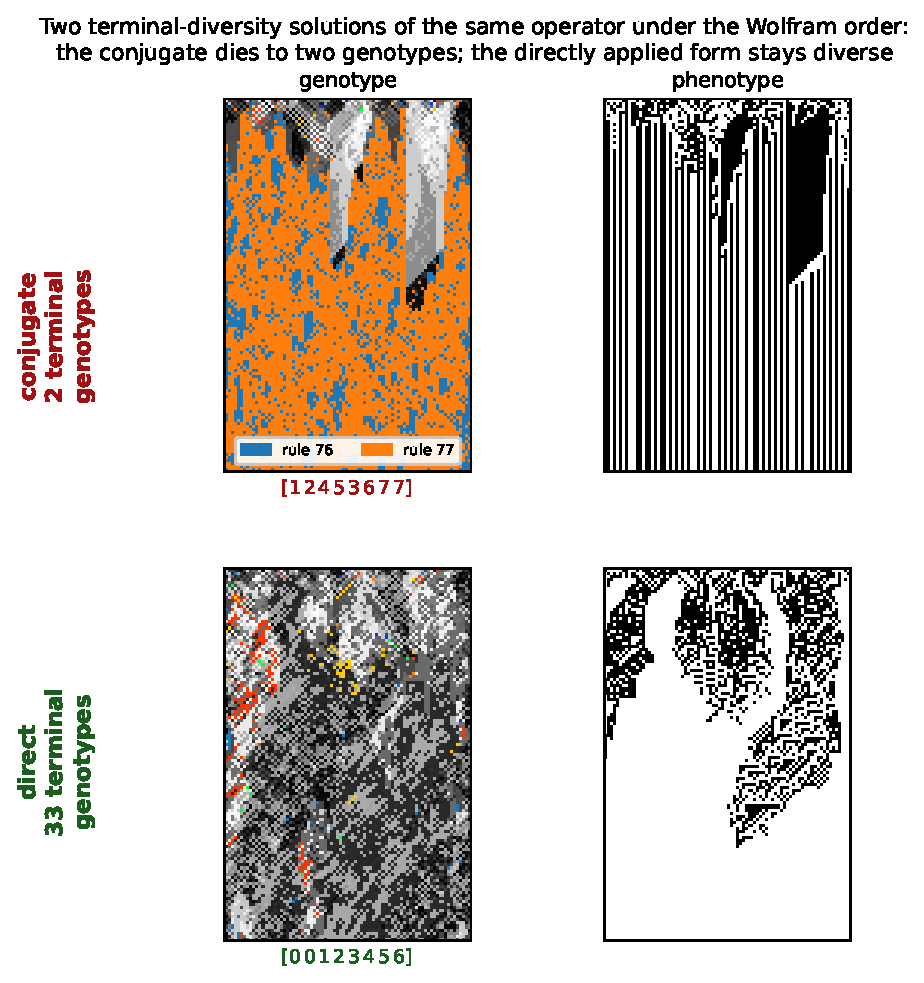
\includegraphics[width=0.82\linewidth]{figures/fig2pair.pdf}
\caption{\textbf{Two terminal-diversity solutions of one historical operator.} The
historical write $[0\,0\,1\,2\,3\,4\,5\,6]$ has two forms under the standard
Wolfram order. Its \emph{conjugate} $[1\,2\,4\,5\,3\,6\,7\,7]$ (top) reproduces the
two-rule behaviour: the genotype collapses to exactly two terminal rules---76 and 77,
adjacent, differing in a single bit---regardless of seed, while the phenotype stays
regular. Applied \emph{directly} (bottom), the same operator keeps a diverse
genotype (${\sim}30$ terminal rules). Two ends of genotypic
aliveness from one historical write.}
\label{fig:fig2pair}
\end{figure}


A cellular automaton normally evolves a field of \emph{states} under one
fixed rule. Here each cell also carries a \emph{rule}, and local writes evolve
that rule field alongside the phenotype. We display an elementary cellular
automaton (ECA) rule in Wolfram order,
\[
111,110,101,100,011,010,001,000,
\]
and index these displayed positions from left to right by $p=0,\ldots,7$.
Thus position $0$ is the $111$ output and most significant bit, while position
$7$ is the $000$ output and least significant bit. Throughout, the indices of
$\sig$, $w$, $g$, and $\bit{p}$ are these \emph{displayed positions}, not the
binary values of the neighbourhoods. If $n\in\{0,\ldots,7\}$ is a numerical
neighbourhood value, its rule output is therefore $g(7-n)$. (The 2015
implementation used the order $000,001,010,100,011,101,110,111$; permutations
quoted from it are conjugated into the displayed order before being named ---
offset $+2$, and so on.)

We study the operator $P_\sig$, parameterised by a permutation
$\sig\in S_8$ of the displayed positions. Writing the displayed byte as a map
$g\colon\{0,\dots,7\}\to\{0,1\}$, the operator sends $g$ to $P_\sig g$ defined by
\begin{equation}
(P_\sig\, g)(q) \;=\; \lnot\, g\bigl(\sig^{-1}(q)\bigr),
\qquad\text{equivalently}\qquad \bit{\sig(p)} := \lnot\,\bit{p}.
\label{eq:prop}
\end{equation}
Each output bit is one input bit, at the position $\sig$ moves it to, negated;
$P_\sig$ is thus a permutation of the eight coordinates composed with a global
complement. The truth table is thereby itself an eight-cell automaton whose
wiring is $\sig$ and whose update is Boolean negation --- an automaton inside
the automaton. Equation~\eqref{eq:prop} defines a family of $8! = 40{,}320$
operators that is finite, exhaustively enumerable, and, as we show below,
exactly classified; Worked example~1 traces one member of the family bit by
bit.\suppnote{\supptheorytext{Definition~1}{Writings, elementary writes, and propagators} \supptheorytext{Observation~1}{Permutations form a small bijective core} \supptheorytext{Worked example~1}{A simultaneous propagator by hand}}

The simultaneous operator of Equation~\eqref{eq:prop} acts on one eight-bit
rule; the spatial experiments place its \emph{elementary} writes---one
truth-table coordinate at a time---inside a two-layer automaton whose cells
hold rules as well as states.\suppnote{\supptheorytext{Definition~2}{Genotype and phenotype} \supptheorytext{Worked example~2}{One site, one complete MetaCA step}}
That substrate is not itself new \parencite{corneli2015search}; what we study
is the operator, understood as an enumerated, exactly classified family---the
object \secref{sec:related} placed against its neighbours.

Figure~\ref{fig:regimes} gives a first measured example of what the operator
choice controls, and it is not a transient of the displayed horizon: under
$\sig=16250374$, Rule~110 holds a median $46\%$ of the genotype at step
$1000$ (six seeds, range $38$--$54\%$), with medians between $39\%$ and
$48\%$ across lattice widths $60$--$480$, while under $\sig=10275364$ it is
absent at the same horizon. These frequencies establish operator-dependent
concentration on Rule~110 in the tested runs; they do not establish a
general preference for computationally distinguished rules.

\begin{figure}[htbp]
\centering
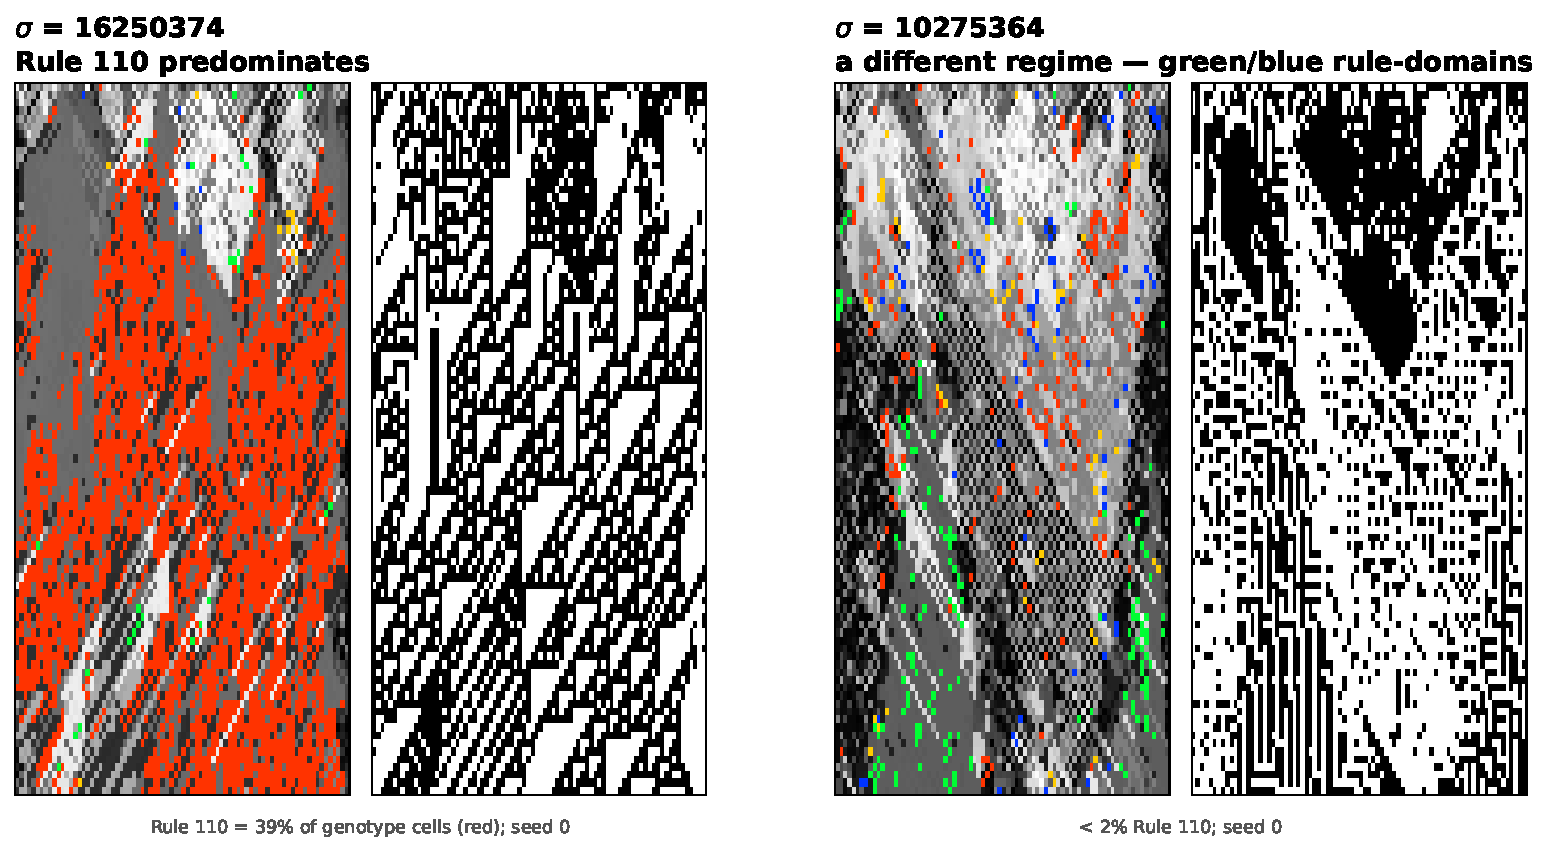
\includegraphics[width=\linewidth]{figures/rule110_spread.pdf}
\caption{Two operators from the family, each shown over time as genotype
(256-colour, left) and phenotype (black and white, right). Under
$\sig = 16250374$ the genotype field comes to be dominated by ECA
Rule~110---the red cells, $39\%$ of the genotype at the representative seed
($35\%$ over six seeds)---and the phenotype accordingly displays Rule~110's
characteristic gliders; under $\sig = 10275364$ a different regime of
rule-domains forms (green and blue, under $2\%$ Rule~110). The
concentration persists and sharpens: at step $1000$, Rule~110 holds a median
$46\%$ of the genotype across six seeds (range $38$--$54\%$), with medians
between $39\%$ and $48\%$ at widths $60$--$480$, while under
$\sig = 10275364$ it vanishes entirely. Genotype
colours follow the 2015 implementation's palette.}
\label{fig:regimes}
\end{figure}

\section{Fixed Rules Exist Exactly When Every Cycle Is Even}
\label{sec:classification}

$P_\sig$ has a fixed rule if and only if every cycle of $\sig$ has even length;
since a one-cycle is odd, this already forces $\sig$ to be fixed-point-free.\supptheory{Theorem~1}{Fixed points and even cycles}

\noindent A fixed rule is a $g$ invariant under~\eqref{eq:prop}, i.e.\ a
$\sig$-equivariant Boolean colouring with $g(\sig k) = \lnot\,g(k)$.
Follow a cycle of length $L$: equivariance forces
$g(k) = (\lnot)^{L} g(k)$, and $(\lnot)^{L}$ is the identity exactly when
$L$ is even; conversely, colour each orbit by the parity of its distance
from a chosen representative. A one-cycle of $\sig$ ($L=1$) is odd and so
admits no such colouring, which is why even cycles are required throughout.

Worked example~3 shows the theorem on the offset-$+2$ operator. The
same small calculation also makes the later $2^k$ count and forced
$\lambda=1/2$ balance visible before we state them generally.\supptheory{Worked example~3}{Even and odd cycles}

This is the signed-cycle fixed-point theorem of Boolean-network theory
\parencite{aracena2008maximum} specialised to~\eqref{eq:prop}: our operator
is a Boolean network whose signed interaction digraph is $\sig$ with every
arc negative, a negation-cycle of length $\ell$ has sign $(-1)^\ell$, and
an isolated negative cycle admits no fixed point while a positive (even)
one admits exactly two. We contribute a machine-checked proof of the
specialised statement in Lean~4 / Mathlib.\footnote{%
\texttt{DarkTower/Patterns/Propagator.lean}, theorem
\texttt{hasAlternatingColouring\_iff\_cycleType\_even}; \texttt{lake build}
clean, no \texttt{sorry} or \texttt{axiom}.}

\subsection{All-even permutations are $105^2$ of $40{,}320$}

The number of $\sig \in S_{2n}$ with all cycles even is $((2n-1)!!)^2$, with
exponential generating function $\sum_n ((2n-1)!!)^2 x^{2n}/(2n)! =
1/\sqrt{1-x^2}$ (the ``set of even cycles'' construction).
For $S_8$ this is $105^2 = 11{,}025$ of $40{,}320$, or $27.34\%$. The count
is classical: it is \textcite{oeis_a001818} and appears as
\textcite[Problem~5.34(c)]{stanley1999enumerative} and in
\textcite{riordan1968combinatorial}. We claim it only as the enumeration of
our operator family, not as a new identity.

\subsection{Fixed bytes number \texorpdfstring{$2^k$}{2 to the k}}

An all-even $\sig$ with $k$ cycles therefore has exactly $2^k$ fixed bytes, and any
$\sig$ with an odd cycle has none.\supptheory{Corollary~1}{The $2^k$ count}
Each even cycle admits exactly two alternating colourings, chosen independently
across cycles, whence $2^k$; the zero case is Theorem~1. This too
is machine-checked.%
\footnote{\texttt{alternatingColouring\_card\_eq\_two\_pow\_cycleType\_card}.}
Summed against these weights the family is consistent:
$\sum 2^{k}$ over all-even $\sig$ equals $(2n)! = 8! = 40{,}320$, the total
number of fixed bytes across the family.

\section{Every Fixed Point Is Balanced}
\label{sec:lambda}

Every fixed point of every operator in the family has exactly four one-bits---equivalently,
Langton's activity parameter is pinned at $\lambda = 4/8 = 1/2$.\supptheory{Theorem~2}{Every fixed point is balanced}

\noindent By Theorem~1 each cycle has even length $2m$; an
alternating colouring assigns such a cycle exactly $m$ ones; summing over
cycles gives $(\sum L)/2 = 8/2 = 4$.\supptheory{Definition~3}{Langton's activity $\lambda$} Exhaustive enumeration confirms it:
across all $40{,}320$ operators and all their fixed points, every one has
Hamming weight four, with zero exceptions.\supptheory{Observation~2}{Balance is a truth-table property} The statement is machine-checked
for $\mathrm{Fin}\,8$.\footnote{%
\texttt{alternatingColouring\_true\_card\_eq\_four}: the true-cells and
false-cells are put in bijection by $\sig$, forcing each to number four.}

We are deliberate about the standing of this result. Langton's critical
value was obtained empirically, as a statistic over rule space
\parencite{langton1990computation}, and its status as an order parameter
was contested: \textcite{mitchell1993revisiting} refuted
\textcite{packard1988adaptation}'s specific genetic-algorithm clustering
claim, not the definition of $\lambda$, which survived as one axis among
others such as Wuensche's $Z$ \parencite{wuensche1999classifying}. There is
a folklore intuition for why $1/2$ is special --- binomial sampling variance
$\lambda(1-\lambda)$ is maximal there --- and it is not ours; and it has been
noted that $\lambda$ alone does not fix a rule's dynamical class, distinct
classes coexisting at a single value \parencite{sakai2002edge}. What
Theorem~2 adds is narrower and firmer than any of these: under
the complementation in~\eqref{eq:prop} the value $1/2$ is \emph{forced} as an
algebraic matter, because any alternation-under-complement colouring is
balanced by parity. We claim balance, exactly; any connection of that
balance to dynamical behaviour we treat as interpretation, not as part of the
theorem.

\subsection{Many distinct survivors, one activity value}

Under an all-even $\sig$, the fixed points of $P_\sig$---the rules it maps to themselves---number $2^k$, where $k$ is the number of cycles of $\sig$ (\secref{sec:classification}). In the spatial runs these are
the rules onto which the field is observed to settle. Every one has
$\lambda = 1/2$ (Theorem~2), so the observed terminal
population is a cast of \emph{distinct} rules---distinct truth tables---sharing
a \emph{single} activity.

The smallest nontrivial case of the count is a single cycle, $k = 1$: two
survivors. The 2015 paper's Figure~8 also exhibits a two-rule residual, but not
an instance of this count: its writing is non-bijective (\secref{sec:object})
and admits no fixed rule at all, so its residual is a hunt on a single
unsettleable position rather than a pair of fixed points.

That die-off curve---the count of distinct rules present over time---is a
natural population-level companion to $\lambda$. Where $\lambda$ is a scalar
assigned to a single rule, this curve is a property of the whole field's
trajectory; and where $\lambda$ is uninformative here---every fixed point
sits at $1/2$---the curve still varies, because it measures the population
rather than the point. We use it cautiously, as an observable rather than an
established order parameter, to tell the rotations whose fields stay diverse
from those whose fields collapse (\secref{sec:interrupter},
Figure~S3.3).

The observed fields can therefore contain several distinct rules even though every fixed rule has the same activity value, $\lambda=1/2$. Terminal rule diversity and fixed-rule activity describe different properties of the field; the causal tests of \secref{sec:causal} examine whether either predicts perturbation reach.


\subsection{A dead genotype can carry a live phenotype}
\label{sec:shell}

The balanced shell is a definite object: exactly $\binom{8}{4} = 70$ rules
carry four active outputs, and by Theorem~2 the absorbing set of
every operator in the family lies wholly inside it. Collapse is therefore not
merely a loss of diversity but a fall onto this particular $70$-rule balanced
shell at $\lambda = 1/2$.

Balance is necessary for a genotype to freeze and silent about what the frozen
rule then does. Run each of the $70$ as an ordinary elementary CA and they
split: $32$ are phenotypically live---sustained change under iteration, the
additive rules $90$, $105$, $150$ and the class-IV rule $54$ among them---while
the rest fall quiescent. The two halves share a single $\lambda$; this is,
inside our family and by construction rather than by survey, the coexistence of
dynamical classes at one activity value that has long been urged against
$\lambda$ as an order parameter \parencite{sakai2002edge}. A field can thus die
in its genotype while the surviving rule keeps its phenotype in motion.

Figure~\ref{fig:shell} is such a field, built to specification. To seat a
collapse on a chosen live rule $R$ it suffices to pair $R$'s four active
positions with its four inactive ones as an involution: four transpositions, an
all-even operator that holds $R$ among its fixed points (Theorem~1).
Whether the field actually settles onto that fixed rule is a separate, dynamical
question (as \secref{sec:interrupter} stresses); here it does. Carried out for
Rule~$54$ this yields
$\sig = [2\,3\,0\,1\,5\,4\,7\,6]$; run from a random field it drives the
genotype to near-uniformity---two rules survive---while the phenotype never
settles. The field has died onto Rule~$105$, another live tenant of the same
shell, whose additive dynamics keep the black-and-white panel full of
structure. Genotypic death and phenotypic death are not the same event.

One caveat marks the open edge of this. An involution fixes not its target
alone but the whole shell compatible with its pairing, and which tenant a
random field actually reaches is set by the basins, not by the construction: we
aimed at $54$ and the dynamics preferred $105$. Existence is settled---live
survivors are constructible---but \emph{steering} a field onto a named rule is
not.

\begin{figure}[htbp]
\centering
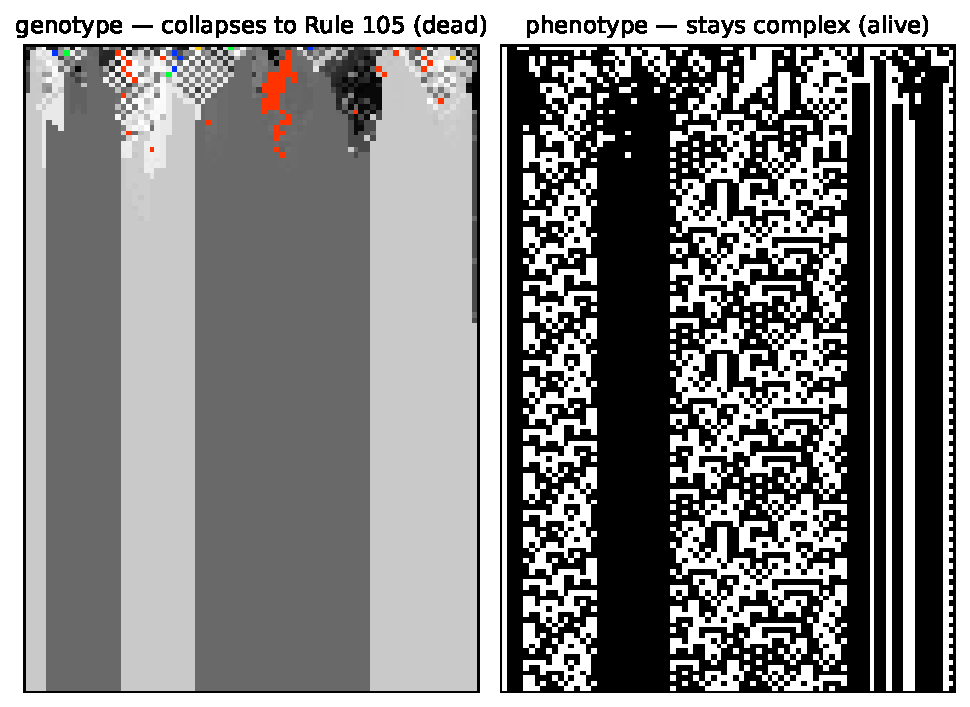
\includegraphics[width=0.82\linewidth]{figures/critical_shell.pdf}
\caption{A genotypically dead, phenotypically live field. The all-even operator
$\sig = [2\,3\,0\,1\,5\,4\,7\,6]$, built to fix the balanced shell containing
Rule~$105$, collapses the genotype (left, 256-colour) to near-uniformity within
a few dozen rows---two rules survive---yet the phenotype (right) never settles:
the field has died onto Rule~$105$, an additive $\lambda = 1/2$ rule whose
dynamics keep it complex. By Theorem~2 every fixed rule of every
operator in the family is balanced, so collapse in this family is always onto
the $70$-rule $\lambda = 1/2$ shell; which tenant a field dies onto, and
whether that tenant's phenotype lives, the theorem does not say. Seed~$1$,
$W = 80$, $T = 120$.}
\label{fig:shell}
\end{figure}

\section{Odd-Cycle Operators All Live; All-Even Types Split}
\label{sec:census}

\subsection{Fixed points make settling possible, not inevitable}

Theorem~1--2 concern fixed bytes; the spatial dynamics adds stochastic elementary writes and, in the census, neighbour blending. In a neighbour-blend step, each truth-table coordinate of a cell's rule is updated from the corresponding coordinates of the left, centre, and right rules: agreeing outer values are copied, while disagreement is resolved by applying the centre rule to that three-bit neighbourhood. Figure~\ref{fig:parity} shows why fixed-point existence is not itself
a dynamical verdict: without blending, all-even rotate$+2$ settles within the
run while all-even rotate$+1$ remains diverse; the odd-cycle examples, which
lack fixed bytes, also remain diverse. The full census below
(\secref{sec:full-census}) makes this quantitative over all $40{,}320$ operators
(Table~\ref{tab:census}); the dynamical content is the \emph{death-rate
difference} between the classes, not the class sizes.

\begin{figure}[htbp]
\centering
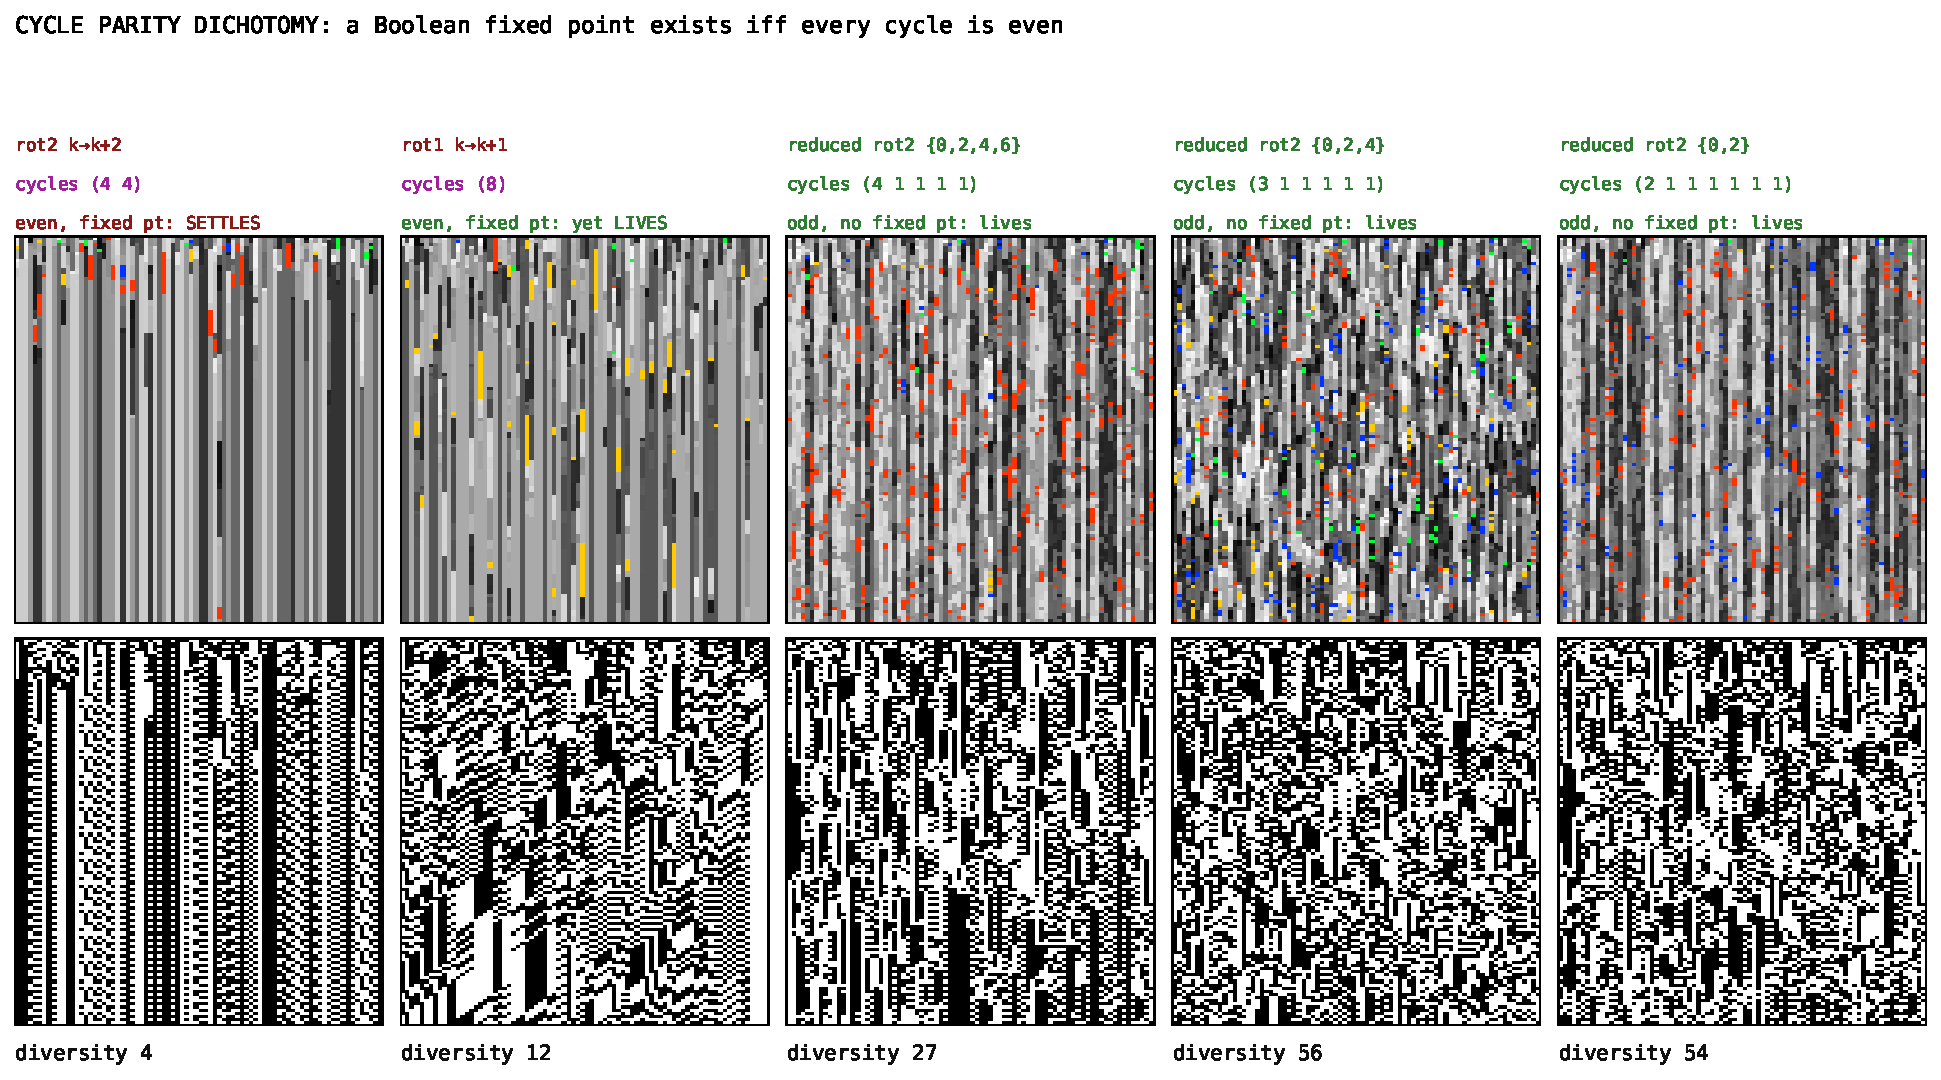
\includegraphics[width=\linewidth]{figures/parity-dichotomy.pdf}
\caption{The parity dichotomy, by example (the census of all $40{,}320$
permutations is summarised in the text). Five operators as genotype (top) and
phenotype (bottom) over time. \emph{Left:} both all-even operators possess fixed
bytes (Theorem~1), but only rotate$+2$ settles within the run,
reaching its $2^k=2^2$ fixed rules; the single-8-cycle rotate$+1$ remains active
at diversity $12$. \emph{Right:} the odd-cycle operators
(reduced rotate$+2$, acting on a subset so the remaining positions are odd
one-cycles) possess no fixed byte and stay diverse in these runs. All five use
stochastic elementary writes without neighbour blending. The figure therefore
illustrates the theorem's fixed-byte classification while also showing that
all-even parity makes settling possible, not inevitable on a finite horizon.}
\label{fig:parity}
\end{figure}

\subsection{A prediction met: no fixed points, no die-off}

To guard against reading structure into a completed enumeration, we fixed a
prediction before running the case. The reduced $\text{rotate}{+}2$
operators act as a single even cycle on a subset of positions and leave the
remaining positions as one-cycles; by that leftover they are \emph{not}
all-even, so by Theorem~1 they possess no fixed point and
should fall on the no-fixed-points side of the dichotomy---no rule for the
field to settle onto, and correspondingly less extinction. They do
(Figure~\ref{fig:parity}, right): they stay diverse rather than dying off.
Absence of fixed points forbids settling onto a single rule; it does not
forbid short-period behaviour, and we claim only the observed persistence of
diversity, not literal aperiodicity.

\subsection{Collapse grows with the number of cycles}
\label{sec:full-census}

The trend becomes an exhaustive finite-run observation once every operator is tabulated. Within the all-even class the specific permutation, not its cycle type alone, decides: two operators of identical two-4-cycle type reach opposite fates (Figure~S3.4), so dynamical class cannot be read off cycle type---what the census quantifies is how each class splits.\supptheory{Definition~4}{Census protocol and aliveness} We ran all
$40{,}320$ permutation-propagators and grouped them by cycle type
(Table~\ref{tab:census}).\suppfinding{1}{The full permutation census}

\begin{table}[t]
\centering\small
\caption{Genotype-alive fraction by cycle type under the census protocol, over
all $40{,}320$ permutations. Any odd cycle forbids a fixed byte
(Theorem~1); empirically, every such operator is alive. The
all-even types split, with collapse becoming more frequent as the number of
cycles $k$ increases.}
\label{tab:census}
\begin{tabular}{lrr}
\toprule
cycle type & count & genotype-alive \\
\midrule
any type with an odd cycle (17 types) & $29{,}295$ & $100.0\%$ \\
$[8]$        & $5{,}040$ & $82.9\%$ \\
$[2\,6]$     & $3{,}360$ & $70.0\%$ \\
$[4\,4]$     & $1{,}260$ & $66.7\%$ \\
$[2\,2\,4]$  & $1{,}260$ & $49.2\%$ \\
$[2\,2\,2\,2]$ & $105$   & $25.7\%$ \\
\bottomrule
\end{tabular}
\end{table}

\section{Fixed Points Are Not Attractors}
\label{sec:interrupter}

Possessing a fixed point (Theorem~1) is not the same as
reaching one, and $P_\sig$ does not by itself move a rule toward
$\lambda = 1/2$.\supptheory{Worked example~4}{Reading the rotation survey} Because $P_\sig$ complements every bit,
$\lambda(P_\sig g) = 1 - \lambda(g)$: the operator \emph{reflects} activity
across $1/2$, exactly preserving the distance $\lvert\lambda - 1/2\rvert$
rather than contracting toward it. And because $P_\sig$ is a bijection on
bytes, a generic rule lies on a periodic orbit and simply cycles---its fixed
points are fixed, but they are not attractors and have no basins. The only
rules pinned at $\lambda = 1/2$ are the fixed points themselves. Attraction in
the experiments therefore belongs to the stochastic elementary-write dynamics,
with or without neighbour coupling, rather than to iteration of the simultaneous
map $P_\sig$.\suppfinding{2}{The rotation survey}

\section{Alternating Two Collapsing Operators Sustains a Diverse Field}
\label{sec:braiding}

Everything so far has held one operator fixed for the length of a run. Relaxing
that---alternating the elementary spatial updates of two operators from step to
step, rather than composing them into a single map---turns out to be
constructive rather than merely destructive, and it is the first place in the
paper where a schedule does something neither of its constituents can.

Braiding two operators that each collapse alone can sustain the
field.\suppnote{\supptheorytext{Definition~5}{Temporal braid} \suppfindingtext{3}{A braid of two collapsing operators can sustain the field}}
Figure~\ref{fig:braid} shows the case: offset~$+2$ (two 4-cycles) and
offset~$+4$ (four 2-cycles) are each genotypically dead run on their own, and
alive when braided. The schedule is also a usable control rather than a
switch. Mixing a sustaining operator with a collapsing one in fixed proportion
over a periodic twelve-step schedule moves late-window rule diversity smoothly
with the mixing fraction (Figure~S3.5), which is what later lets us
treat diversity as a dial to be turned rather than a property a run happens to
have.\suppfinding{4}{The mixing fraction is a reproducible diversity control}

\begin{figure}[htbp]
\centering
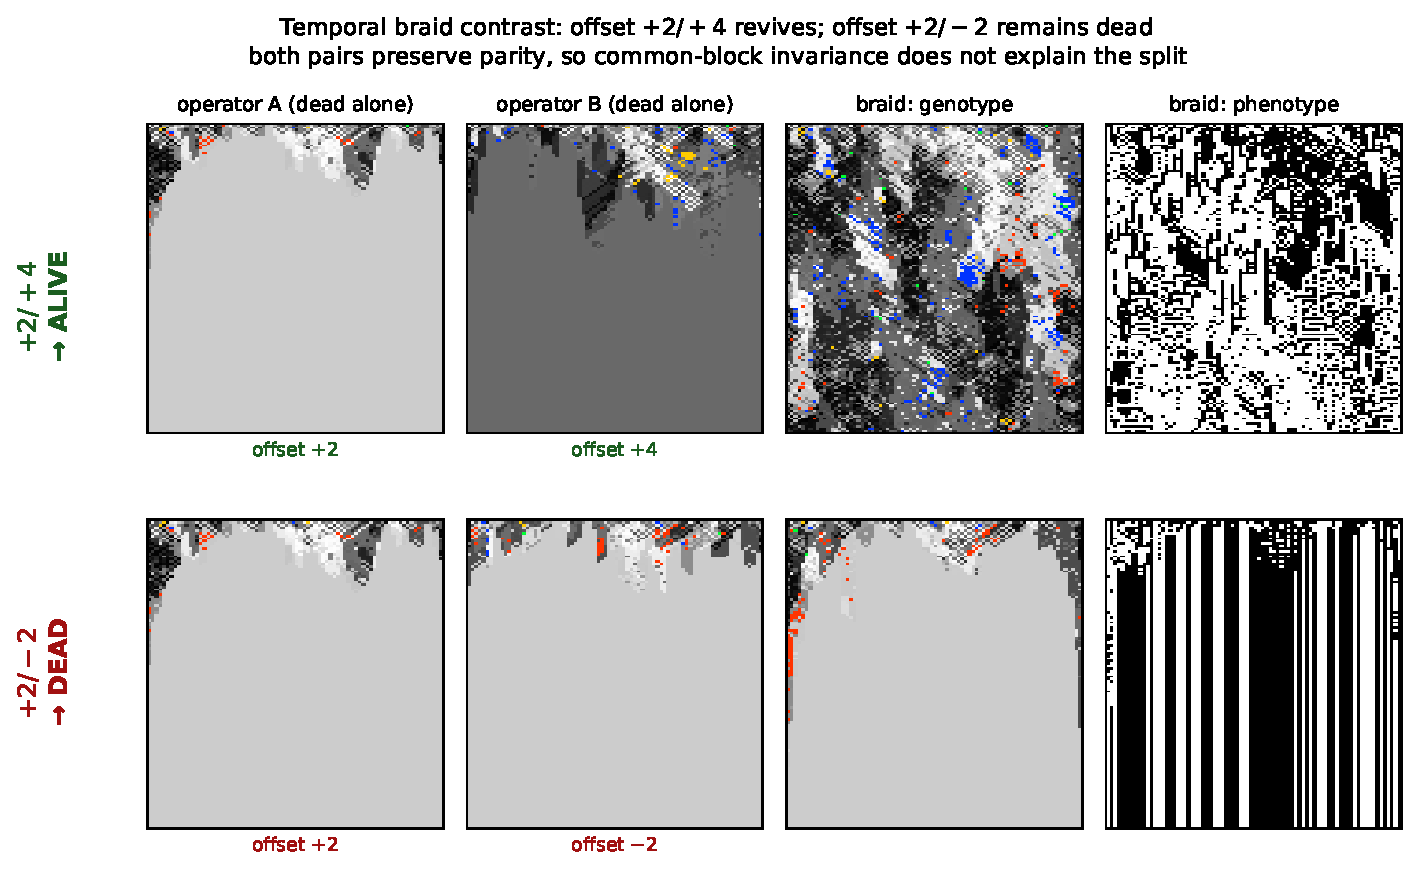
\includegraphics[width=\linewidth]{figures/braid.pdf}
\caption{\textbf{Temporal braiding can sustain aliveness.} Two operators that each collapse
alone are braided by alternating their elementary spatial updates. Top:
offset$+2$ (two
4-cycles) and offset$+4$ (four 2-cycles) are each genotypically dead, yet their
braid is alive (genotype change-rate $0.76$, vs.\ $0$ for either alone). Bottom:
offset$+2$ braided with offset$-2$ stays dead. Both tested pairs preserve parity,
so the contrast is not explained by the existence of that common invariant
partition. The result concerns time-dependent coupled dynamics, not composition
of the simultaneous maps $P_\sigma$.}
\label{fig:braid}
\end{figure}

Each operator negates every bit, so under composition the flips cancel in pairs: a product
of two is a \emph{pure} coordinate permutation with no negation left.\supptheory{Proposition~1}{Composition parity}

Exploratory searches over products of two and three simultaneous propagators
found no additional structural regime.\supptheory{Definition~6}{Interrupter}
Algebraic composition is therefore closed in the sense of
Proposition~1. Temporal braiding is a different operation: it
alternates stochastic elementary writes inside the spatially coupled dynamics
rather than replacing them by one composed map, retaining each intermediate
coupled state, which is why the braids of \secref{sec:braiding} can produce
dynamics absent from either held operator.\suppfinding{5}{The rotation split occurs with and without neighbour blending}
The second constructive mechanism---pairing a propagator with a
phenotype-reading step---is the subject of Part~II.

\section{A Broad Crossover and No Critical Point}
\label{sec:discussion}

The survey (Figure~S3.1) exposes a sharp behavioural split within a
family of provably fixed-point-bearing operators: only the single 8-cycles
(offset $\pm 1$, $\pm 3$) sustain a high-diversity phase, while offset $\pm 2$ and
$\pm 4$ collapse. A reader is entitled to ask whether that phase sits at a
\emph{critical point}---tuned between an ordered and a disordered phase, as CA
complexity is often supposed to \parencite{langton1990computation}. This is the
first of the two readings distinguished at the outset---an edge of chaos located
in \emph{parameter space}, at some value of a tunable control parameter---and
the finite-size scan below is the test of it, the only place in this paper where
that reading is put to the question. \suppfinding{6}{No finite-size evidence of a critical point over the tested range}

Figure~\ref{fig:phase} collects the four diagnostics. The scan is over the
propagator fraction $q$, from all blend at $q=0$ to all propagator at $q=1$, at
lattice widths $L = 30$ to $240$ with $32$ seeds each; the point of varying $L$
is that a genuine transition sharpens as the system grows while a crossover does
not. Genotype activity fits a logistic in $q$ at every size ($R^2 > 0.99$), but
the crossover width does not shrink over these sizes ($w \sim L^{-0.04}$). The
size-scaled run-to-run spread $L\,\mathrm{Var}(a_G)$, used here as a
susceptibility proxy, does peak inside the crossover and grows about $5.7$-fold, but
its maximum wanders---from $q=0.75$ to $0.50$ and then to the sampled boundary
$q=1$ for the two largest sizes---rather than settling. Finite-horizon collapse
becomes rarer with size, and the Binder cumulant has no common crossing. Each
diagnostic is individually consistent with a critical point; none of them
locates one, and together they support a broad crossover instead.

\begin{figure}[htbp]
\centering
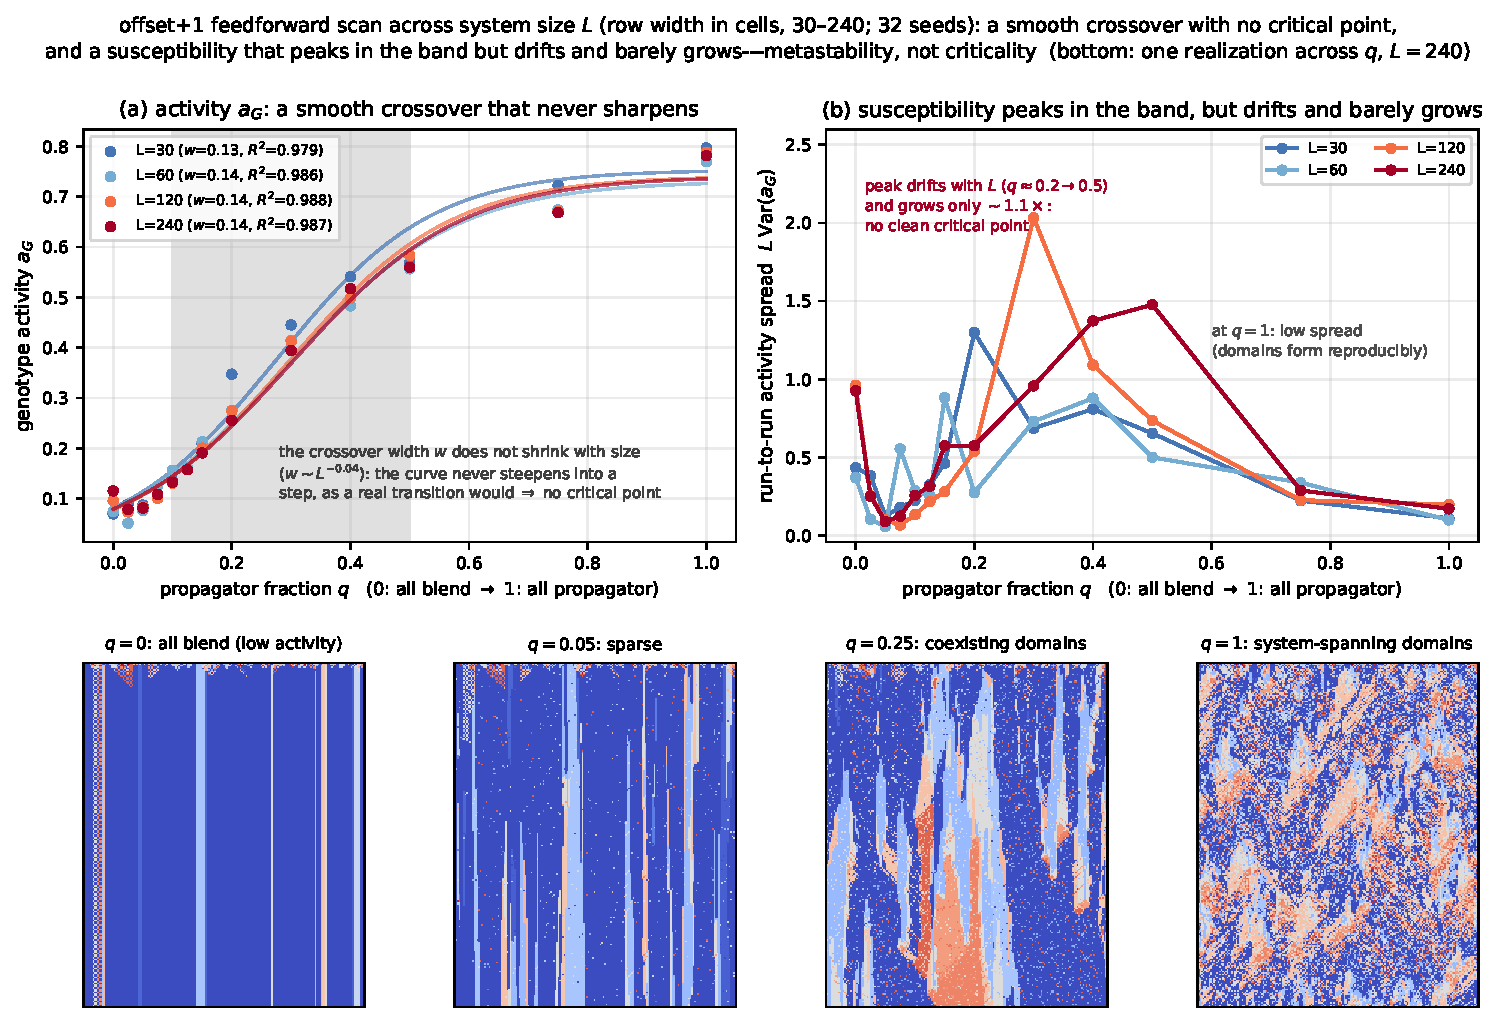
\includegraphics[width=\linewidth]{figures/eoc_phase.pdf}
\caption{\textbf{Finite-size scan across the propagator fraction.}
Offset $+1$ without phenotype feedback, $L = 30$--$240$, $32$ seeds per size.
\textbf{(a)}~genotype activity with logistic fits; \textbf{(b)}~size-scaled
spread as a susceptibility proxy; \textbf{(c)}~finite-horizon collapse
frequency; \textbf{(d)}~the Binder cumulant. Bottom: one paired realisation at
$L = 240$ tinted by isolated-rule activity.}
\label{fig:phase}
\end{figure}

\newpage
\part{Beyond the Permutation Core: Feedback and Causal Propagation}
\label{part:feedback}

This part establishes the paper's measurement and what it finds. The
instrument: flip one cell, fork the run, and measure how far the difference
between the two copies travels, calibrated against elementary rules of known
behaviour. On that instrument, architectures whose rule updates read the
current phenotype roughly double the reach of matched architectures that do
not; a dial replacing a growing fraction of current readings with readings of
a frozen copy---itself a real phenotype, so spatial statistics match at every
setting---reduces reach smoothly; and sustained rule diversity, mutation,
refuges, niches, and rule mobility leave reach unchanged, while a
conservative transport that only moves rules from place to place raises it.
What moves reach is current state information reaching the rule layer;
diversity of the rules themselves is inert. The part closes by recovering the
same ordering from an independent construction: a gate deciding locally when
rewriting fires reproduces the prescribed-rate dial when blind to cell
states, exceeds it when reading current states, and falls below it when
reading a frozen field of matched statistics and firing rate.

Part~I's classified object and exhaustive census were the finite permutation
core; its temporal braid was the boundary case, already replacing one held
operator with a schedule. We now retain the same genotype--phenotype lattice
and elementary rule semantics but drop the single-operator restriction. The
objects in Part~II are update architectures: time-dependent schedules,
phenotype-conditioned writes, mutation and holding protocols, and conservative
local transports. Some use writings from the $8^8$ family as components, but a
state-dependent architecture is not itself one fixed writing. Consequently,
the results below neither classify nor measure the $8!$ family as a whole; they
test how causal propagation changes when the genotype update can read the
phenotype.

\section{A Construction That Reads Its Own Phenotype Sustains Structured Phenotype}
\label{sec:feedback-construction}

The phenotype-reading step begins from a four-bit context: the local
three-cell phenotype neighbourhood before the update and the cell's newly
computed phenotype bit. From that context it constructs four ordered
candidates: the observed four bits, their full complement, the observed bits
with the second bit flipped, and the observed bits with the first, third and
fourth bits flipped. At each truth-table position it compares the three rule
bits supplied by the left, centre and right cells with the first three bits of
those candidates; the fourth bit of the first match becomes the new rule bit,
and an unmatched position takes the all-zero fallback. We call the composition
of this step with the offset-$+2$ propagator the \emph{river}.
Figure~\ref{fig:river} shows a representative run at $L=240$: alternating
phenotype domains branch, merge and reorganise for the length of the run rather
than resolving to a homogeneous or short-period field, whereas the bare
rotations collapse or cycle.\suppnote{\supptheorytext{Definition~7}{River} \suppfindingtext{7}{The river sustains structured phenotype}}

\begin{figure}[htbp]
\centering
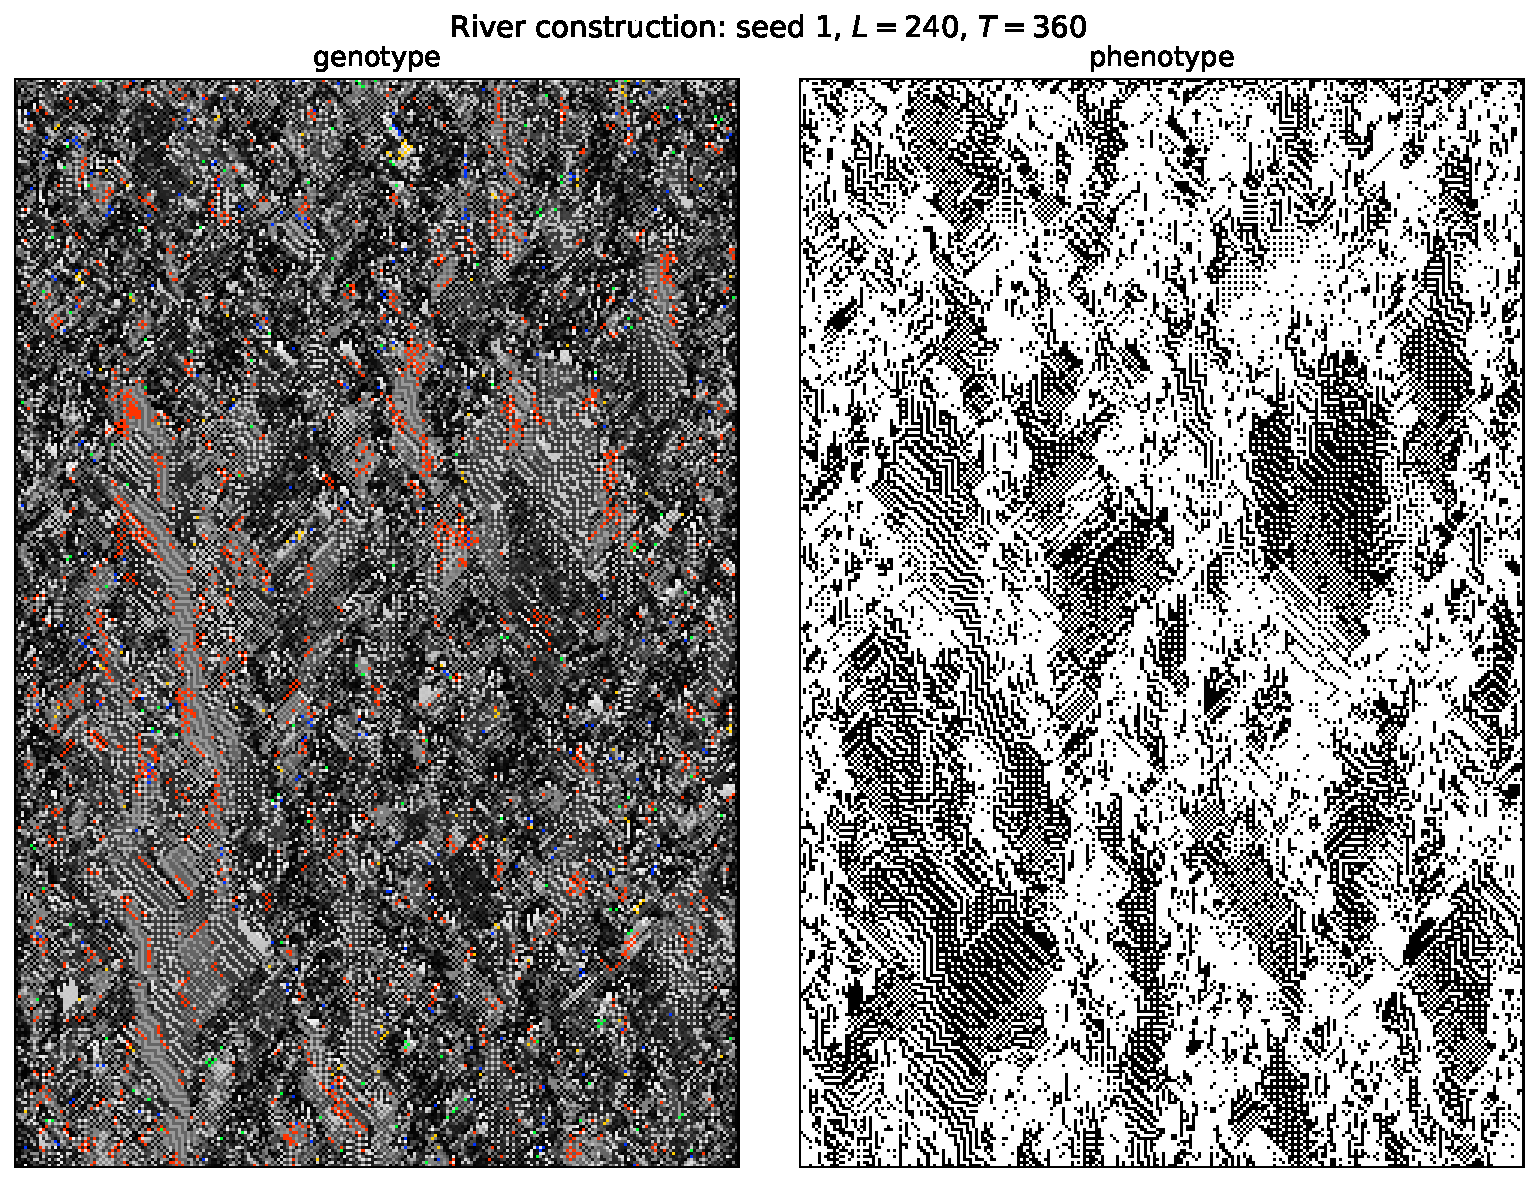
\includegraphics[width=\linewidth]{figures/river.pdf}
\caption{\textbf{A river spacetime plate.} One pinned representative
run (seed 1) at $L=240$, $T=360$, with genotype at left and phenotype at
right. The offset-$+2$ propagator is composed with a phenotype-reading,
four-candidate, first-match template construction (fallback: the all-zero
rule). Alternating phenotype domains branch, merge, and reorganise throughout
the run rather than resolving to a homogeneous or short-period field.
Genotype is coloured by rule as in
Figures~\ref{fig:regimes}--Figure~S3.1: greyscale by byte value, with
well-known ECAs highlighted and red denoting Rule~110. Where the bare rotations
collapse or cycle (Figure~S3.1), this composition sustains structured
phenotype for the length of the observed run.}
\label{fig:river}
\end{figure}

\section{Feedback Roughly Doubles How Far a Flip Travels}
\label{sec:causal}

\phantomsection\label{sec:metrics}%
Two measures were tried before the causal one and neither separated the
regimes. A normalised compression distance on the rule field tracks how many
distinct rules are present rather than how they are arranged, and a
block-entropy estimate over the phenotype is dominated by the same quantity.
Both therefore report diversity, which \secref{sec:diversity-axis} shows is
not the coordinate that governs propagation. That failure is what motivates
measuring a perturbation directly rather than summarising a field.

A causal test also avoids a general problem with observational regions. Any
statistic computed over a region drawn from the field it is computed on invites
circularity, and no null defined only by moving that region can necessarily
detect it. We therefore stop drawing regions: perturb one cell and ask where
the effect arrives.

We run the phenotype-reading construction of
\secref{sec:feedback-construction} to $t^{*}=60$,
fork, flip a single phenotype bit at site $x$, and continue both branches to
$T=120$, recording which cells differ. The fork is exact: the construction draws
one pseudo-random position per cell per step, so re-running from the same seed
gives both branches an identical tape and every divergence is the causal
consequence of the flip. The control is the matched feedback-off variant---same
seed, tape, construction and initial state, with only the live
phenotype-to-genotype edge cut. Figure~S3.6 sweeps the flip over all $80$ sites and records damage at a sequence of horizons.\suppfinding{8}{Phenotype-to-genotype feedback roughly doubles causal reach}

A glider carries a fixed-width
packet at constant velocity; a conductive medium disperses. Tracking the damage
centroid distinguishes them, and the reference values must be measured rather
than assumed---elementary rule $110$, whose gliders support universal
computation, does not give a fixed packet under a random single-site
perturbation, because the perturbation creates and destroys gliders which then
collide.\suppnote{\suppfindingtext{9}{Causal reach on a scale calibrated against elementary rules} \suppfindingtext{10}{The order parameter is the strength of the phenotype-to-genotype coupling}}

Figure~\ref{fig:regime-placement} places every construction on that one axis.
All points share the protocol of \suppfindingref{9}, and the calibration
reproduces rules $0$, $204$ and $90$ exactly against it, so the reference values
drawn from the elementary rules carry over unchanged. The rows split the constructions by
coupling rather than by provenance, and the split is clean. Nothing whose
genotype update is blind to the phenotype clears rule $90$---not even the ungated transport controls, which are fully mobile and
merely cannot see what they are moving through. Everything that reads the
phenotype lands inside. The river composition defined in \secref{sec:feedback-construction} appears in
both rows: its reach is $12.97$ when the genotype update reads the live
phenotype and $5.51$ in the matched control without that live edge. The arrow
therefore compares one construction with and without the measured causal
connection.

\begin{figure}[htbp]
\centering
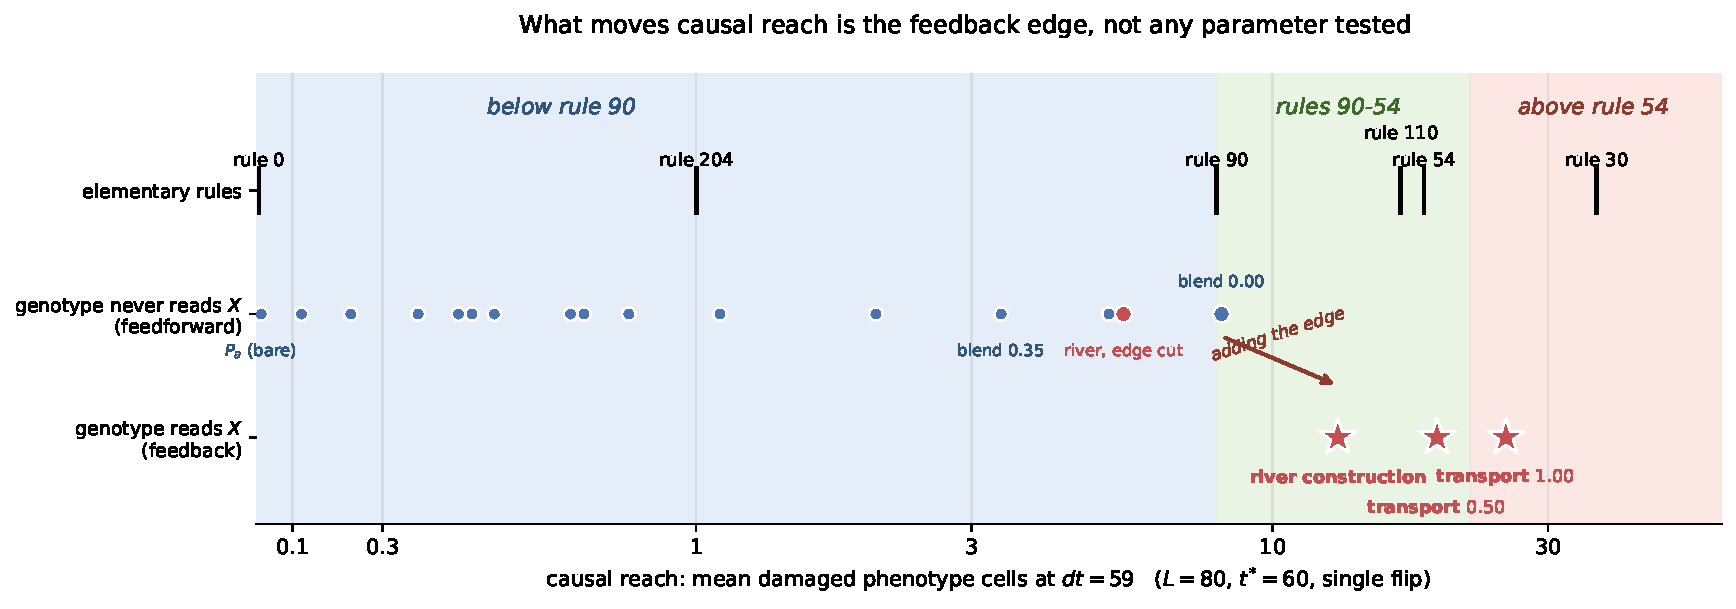
\includegraphics[width=\linewidth]{figures/regime_placement.pdf}
\caption{\textbf{Every construction on one scale.} Causal reach under the
protocol of \suppfindingref{9}. The shaded intervals are named for the
elementary rules that bound them and assert no Wolfram class: rule $90$ is class~III and
sits at the first boundary. Rows divide constructions by whether the genotype update reads the
phenotype. Right: the measurement itself, at the pair the arrow joins---the
same construction, same seed, same flipped cell, with the live edge (damage
cone in red, reach $12.97$) and with the edge cut ($5.51$).}
\label{fig:regime-placement}
\end{figure}

The same sweep also gives the growth of the damage cone and the displacement
of its centroid (Figure~S3.7); we report those exponents
descriptively and draw no inference from them about gliders or particles.

The reach scale separates propagating from non-propagating responses: frozen
rules return exactly zero. It is not a regime coordinate. Wolfram class~III
rules bracket the measured range---rule $90$ at $8.00$ and rule $30$ at
$37.50$---with the class~IV rules $54$ and $110$ between them, so position on
this axis does not classify a system as ordered, complex or chaotic. What the
comparison supports is narrower: on the same fork-and-flip measure, allowing
the river's genotype update to read the live phenotype changes reach from
$5.51$ to $12.97$. Because the protocol draws no observational region, that
comparison does not depend on selecting a region from the field being measured.

\subsection{Reach is monotone in the coupling gain}
\label{sec:gain}

Treating that coupling as present or absent understates it. In both
constructions that read the phenotype it is a quantity, and causal reach is a
graded, monotone function of it.\suppfinding{11}{Coupling is a dial, not a switch, and reach is monotone along it}

For conservative transport the gain is the phenotype-gated swap rate; reach
crosses rule $90$ between rates $0.10$ and $0.20$ and saturates past $0.75$. For
the river it is the \emph{currency} of the phenotype bits the genotype reads:
each cell at each step reads the live phenotype with probability $\gamma$ and a
frozen reference otherwise, so $\gamma$ is the fraction of the genotype's view
that is causally current. Because the frozen field is itself a real phenotype,
marginals and spatial structure are matched at every $\gamma$ and only causal
currency varies; because $\gamma = 1$ reproduces the live river exactly, the
dial is anchored against a measurement made independently of it.

The two frozen conditions capture their reference fields at different times.
For the $\gamma$ dial, one phenotype field is captured before the fork and
supplied unchanged to both branches; at $\gamma=0$, neither branch's genotype
update can read the flipped bit, and reach is $1.28$. The ablated control instead
captures a separate frozen field at the start of each post-fork continuation,
after the perturbation has been applied. Its perturbed branch therefore reads a
static field containing the flip while its unperturbed branch reads a static
field without it, and reach is $5.51$. Thus $5.51$ removes temporal updating but
retains a branch-specific static difference, whereas $1.28$ removes current
phenotype information from the comparison; the full measured span is $1.28$ to
$12.97$.

And the two dials have opposite curvature (Figure~\ref{fig:gain-curves}).
Transport is concave and buys most of its reach early; the river is convex, with
$45$\% of its span in the last eighth of $\gamma$, so one stale read in eight
costs $40$\% of the reach. Monotonicity in the coupling is thus common to both
constructions while its shape is not, and we would not generalise the shape from
two cases.

\begin{figure}[htbp]
\centering
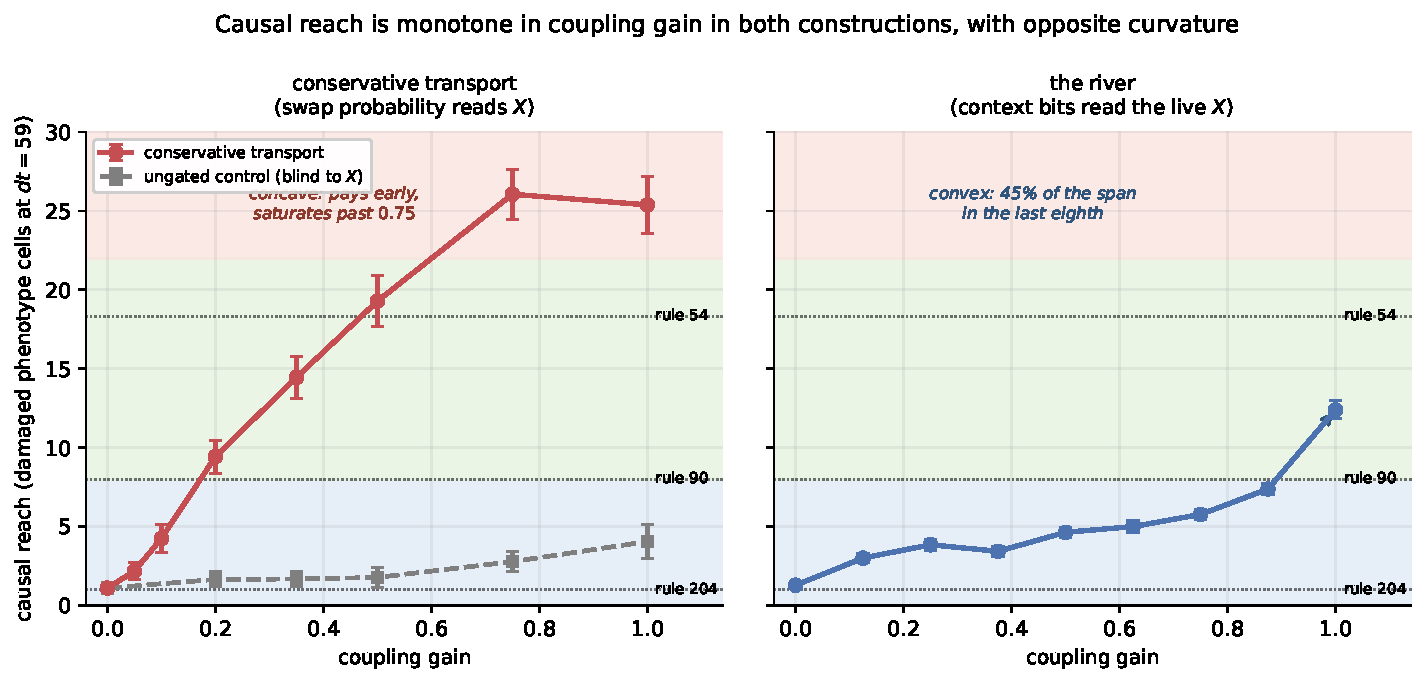
\includegraphics[width=\linewidth]{figures/gain_curves.pdf}
\caption{\textbf{Two couplings, dialled.} Causal reach against coupling gain
for conservative transport (left, with an ungated control at matched mean swap
probability) and for the river (right). Error bars are standard errors.}
\label{fig:gain-curves}
\end{figure}

\subsection{Transport moves reach; diversity does not}
\label{sec:diversity-axis}

That $\lambda$ cannot discriminate among the fixed points is
Theorem~2's point (\secref{sec:lambda}); nor can it be rescued by
computing it on the realized dynamics. Across the nine configurations of
Figure~S3.2 the empirical neighbourhood distribution is close to
uniform---normalised visitation entropy $0.946$ to $0.999$, all eight
neighbourhoods visited in every run---so $\lambda$ read off the realized
transitions ($0.42$ to $0.52$ uniform-weighted, $0.40$ to $0.51$
visitation-weighted) sits near $1/2$ wherever the nominal value does. The
sustained distinct-rule count \emph{can} discriminate, and the causal measure
above lets us ask the stronger question: does causal reach depend on diversity
itself, or on the mechanism used to sustain it?

Our initial survey varied sustained diversity by seven mechanisms that share little: the bare
operator family; braided writings; the fork time after seeding the genotype with
a randomised \emph{full} rule population; a continuous blend strength; random
rule mutation; asynchronous refuges that hold a cell's rule exactly with some
probability; and spatially phase-shifted braid niches. A limiting case anchors
the top of the range: a genotype held fixed at the full population has maximal
diversity and no rewriting at all. The coordinate throughout is diversity
\emph{sustained through the response window}, not diversity at the instant of
the fork---a field seeded with all $256$ rules holds them for one step and
collapses during the very window the damage is measured in.\suppfinding{12}{Sustained diversity does not determine causal reach; conservative transport breaks the apparent interior optimum}

Figure~\ref{fig:diversity-axis} shows why the apparent optimum was an artefact.
The original configurations trace a rise and fall against sustained diversity,
but every point on the descending limb obtains its diversity either by
replacement mutation or by holding rules still, so the descent measures those
two mechanisms rather than diversity. The conservative runs, which hold the rule
histogram exactly invariant while varying transport, separate into flat bands
--- one per transport rate --- that span the whole diversity axis. Reading
across a band shows the effect of diversity at fixed transport and finds almost
none; reading between bands shows the effect of transport and finds an order of
magnitude.

\begin{figure}[htbp]
\centering
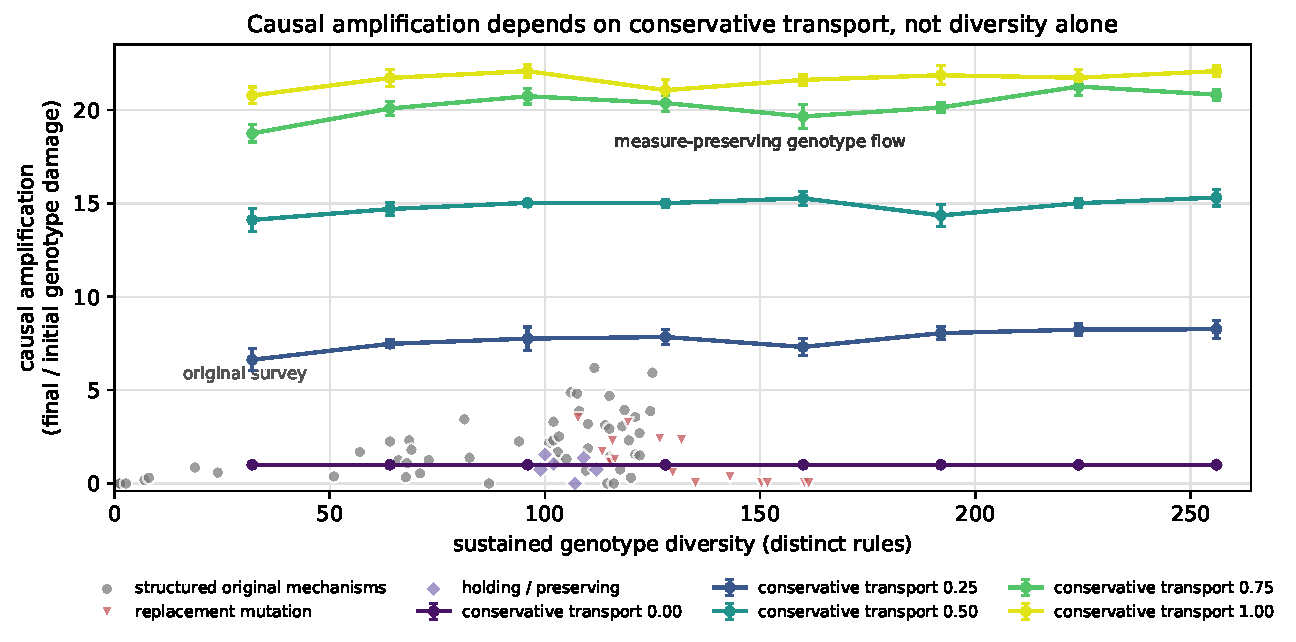
\includegraphics[width=\linewidth]{figures/diversity_axis.pdf}
\caption{\textbf{Causal reach against sustained genotype
diversity.} The original $76$ configurations, grouped by mechanism, with the
conservative-transport runs overlaid as one band per transport rate. The bands
are flat: reading across any one shows the effect of diversity at fixed
transport and finds almost none, while reading between bands shows the effect
of transport and finds an order of magnitude. Diversity does not govern reach;
how the genotype measure is moved does.}
\label{fig:diversity-axis}
\end{figure}

Two cautions bound this result. First, the conservative intervention is a local
transposition, rather than the one-bit, one-site intervention of the original
survey. Normalising by initial damage puts their amplification on a common
scale, but the conservative curves are a falsification control, not a claim
that their absolute heights rank all mechanisms. Second, phenotype-gated
bijective exchange is one deliberately constructed transport law, tested at one
lattice width and one response horizon. It establishes existence: fields can
remain mobile and propagate damage without mutation at sustained diversities
above $135$ distinct rules---the highest diversity any mechanism of the
original survey reaches without replacement mutation or a held genotype
(Figure~\ref{fig:diversity-axis}, grey band; \suppfindingref{12}). It does not establish that transport rate is a universal
order parameter.

The defensible conclusion is narrower and cleaner. Distinct-rule diversity
describes population persistence in the Part~I operator experiments, but it
does not govern causal reach across the Part~II architectures. The latter
depends on how rewriting or transport is organised. Identifying a coordinate
that captures that organisation across mechanisms is work for another paper;
the classification of \secref{sec:classification} guarantees only that
$\lambda$ cannot discriminate among fixed points in the permutation core.



\subsection{The live read is determinative, not a tiebreak}

One measurement bounds how the convexity of \secref{sec:gain} should be read.
Asking, per cell and step, whether the live phenotype context selects a
\emph{different} rule than a frozen context would: it does in $73.1$\% of
cell-steps (and in $76.8$\% against no context), over four seeds at $L=80$ for
$120$ steps. The construction's first-match runs over four candidates, so an
uninformative re-selection would differ in about $75$\% of cases: at $73.1$\% a
frozen context carries almost no information about the live answer. The read is
determinative rather than a tiebreak, which is what a convex gain curve should
lead one to expect, and it means there is no common case that a
phenotype-blind rule could encode in its place. We draw no stronger conclusion
from this than that: whether \emph{any} blind construction could match the
river is a question about a search we have not run, and
\suppfindingref{8} reports only that the sixteen tested ones do not.

\section{A Gate Reading Current States Raises Reach; Reading a Frozen Field Lowers It}
\label{sec:endogenous-gain}

A \emph{conditional composition} applies one operator where a local predicate
holds and another where it does not. Throughout this section the pair is
conservative transport at unit rate ($25.38$ on the \secref{sec:causal}
calibration) and holding ($1.21$); the predicate decides cell by cell, and its
\emph{firing fraction} $f$ is measured from the run. The gain-dial
disciplines of \secref{sec:gain} carry over: the transport stream advances
whether or not the gate fires, and predicate randomness is re-seeded
identically in both branches of a damage fork.

A gate firing at a prescribed rate, blind to the phenotype, is described across
six rates spanning $f = 0.10$ to $0.94$ by a line through the holding value,
%
\begin{equation}
  \mathrm{reach}(f) \;=\; 1.21 \;+\; 22.42\,f ,
  \label{eq:blind-line}
\end{equation}
%
with $R^{2} = 0.993$: a blind conditional composition is \emph{exactly} a
gain dial, its duty cycle playing the role $\gamma$ plays in
\secref{sec:gain}. Letting the condition read the phenotype changes that.
Writing $\mathrm{agree}\,k/m$ for the condition that at least $k$ cells of
the centred circular $m$-cell phenotype neighbourhood agree with the centre,
thirteen such gates spanning widths $m \in \{3,5,7,9\}$ all exceed
Equation~\eqref{eq:blind-line} at their own measured firing fraction; the
widest, $\mathrm{agree}\,5/9$, reaches $38.23$ while firing on only $63\%$
of opportunities---above unit-rate transport's own $25.38$.

Width, however, is also the spatial correlation length of the firing pattern
(neighbouring decisions share $m-1$ inputs), and correlated firing of a
transport operator composes adjacent swaps into longer-range movement on its
own. The \emph{frozen} gate rules that reading out: the identical predicate
applied to the phenotype as it stood at $t^{*}$---same width, same spatial
statistics, a real phenotype field---falls below the blind line in all seven
matched pairs, by $14.5$ cells against its live counterpart on average,
though it fires \emph{more} often in six of the seven. A blind condition
reproduces the dial; a current-reading condition exceeds it; a stale-reading
condition of matched statistics falls below it (Figure~\ref{fig:frozen-gate}).

\begin{figure}[htbp]
\centering
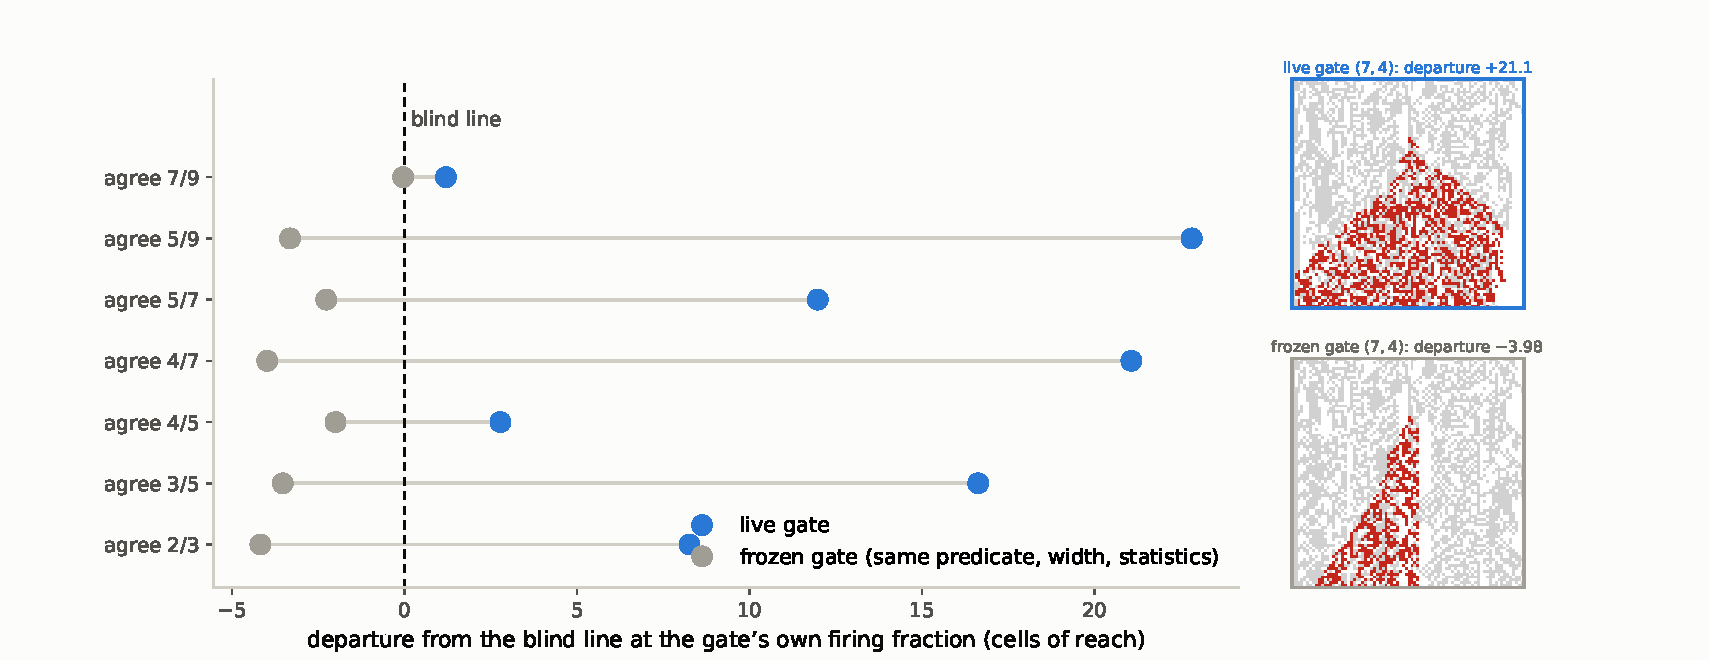
\includegraphics[width=0.9\linewidth]{figures/frozen-gate.pdf}
\caption{\textbf{The frozen-gate control: currency, not correlation.} Departure
from the blind line of Equation~\eqref{eq:blind-line}, at each gate's own
measured firing fraction, for the seven matched $(m,k)$ pairs (sixteen seeds
per row). The live gate exceeds its frozen counterpart in every pair, by
$14.5$ cells on average, and \emph{every} frozen departure is negative,
though the two share predicate, width, and spatial statistics, and the frozen
gate fires more often in six of the seven pairs. What the reading gate
exploits is the causal currency of the phenotype it reads. The
live--blind--frozen ordering therefore recurs in a conditional composition
that uses neither the transport-rate dial nor the river's $\gamma$ dial.
Right: the $(7,4)$ pair's damage fields---the live gate spreads one flip
into a cone; the frozen gate, firing on a field of the same statistics,
confines it to a needle.}
\label{fig:frozen-gate}
\end{figure}

% =====================================================================
% Part III -- Endogenous Coupling and Exotypes.  Draft 2026-08-06 (claude-14).
%
% Scope per Joe, 2026-08-06: Part III explains the exotype layer and reports
% what the search found AT THE END.  The EFE miner -- the apparatus that did the
% searching -- moves to a supplement: it is a tool, not a theory of MetaCAs.
% Update 2026-08-08 (fable): the research question is closed by deterministic
% measurements (TN-part-iii-endogenous-ruling.md, incl. its retraction
% addenda; scripts none_label_check, lstar_tau_measure,
% hetfixed_sheet_reference, boundary_invasion_rescue, boundary_blast,
% morphology_default_check).  Section order follows the discovery order:
% gate -> layer -> vocabulary -> scope -> three outcomes -> closure (last,
% with the combined two-interventions figure).
%
% Labels referenced here that exist in draft7.tex: sec:object, eq:prop,
% sec:classification, sec:census, sec:full-census, sec:gain, part:core.
% =====================================================================

\part{Exotypes}
\label{part:endogenous}

\noindent In Part~II the gain of the phenotype-to-genotype loop is a parameter
we set, and the gate of \secref{sec:endogenous-gain} made the firing
condition a function of the lattice while the operator remained a property of
the run. This part takes the remaining step: the operator itself becomes a
property of the cell.

Its findings, in order. When the operator becomes per-cell state, adopted
between neighbours under a selection rule, three outcomes occur at the tested
parameters: the changing phase (sites whose phenotypes continue to update) eliminates the frozen phase (sites whose phenotypes remain unchanged for fifteen steps), the frozen phase
takes over, or the two persist together for the full horizon. No locally
computable quantity we tested ranks operators well enough to find the third
outcome from within a run. A local intervention built to protect it---cells in
uniform surroundings copying operators from phase boundaries---accelerates
the freezing instead. Undirected noise does prevent freezing, but what it
holds looks different: a foam of small frozen islands amid changing
surroundings (Figure~\ref{fig:interventions}), against the extended frozen
and changing regions of the found configuration
(Figure~\ref{fig:exo-lavalamp}); the measured difference is frozen
fraction, $0.3$ against $0.08$. Finally, with adoption
switched off, none of thirty control runs freezes or dies: the frozen
endpoints are an effect of the adoption rule at high precision, not of the
lattice underneath. Two probes directed by the literature sharpen both
findings: the freeze is nucleation-limited (an established frozen domain
invades, yet the frozen phase never arises from developed churn), and a
one-sided rule that writes only into long-settled cells holds a mixed state
at a sixth of the dose of its randomly placed control --- placement carries
information after all, once the trigger is one-sided.

\section{The Gate Sets the Timing of Rewrites; the Exotype Sets Their Content}
\label{sec:exotype-intro}

The gate of \secref{sec:endogenous-gain} chooses \emph{when} an operator
fires. It does not choose \emph{which}: there the pair of constituents is fixed, and the
predicate selects between them; the permutation $\sig$ supplying the rewriting is
a property of the run.  Each
cell carries its own propagator, drawn from a small named vocabulary and
transmitted between neighbours, so the operator acting at a site becomes part of
the local state.

Whether such a lattice can find its own operating point, using only
quantities available to it at runtime, is the question the remainder of the
part answers. The instrument behind every measurement so far---causal reach,
computed by forking the run and perturbing a twin---is not such a quantity:
no system can fork itself, and reach measures causal propagation rather than
dynamical regime, so it would not by itself say where the system should
arrive.

\section{The Exotype Is a Structured Mutation Operator}
\label{sec:exotype-layer}

An \emph{exotype} is a per-cell assignment of a propagator. The vocabulary is a
set of named permutations $\sig$; the grid holds one name per site; and the
names are transmitted between neighbouring sites by a local policy. Nothing in
the vocabulary is new to this paper---each name denotes a member of the family
Equation~\eqref{eq:prop} defines---but the assignment is new, because $\sig$ has
until now been a property of a run rather than of a cell.

The transition is one elementary write. At a site whose genotype is the
eight-bit rule $g$, with $\sig$ the propagator the site currently carries, a
coordinate $k \in \{0,\dots,7\}$ is drawn uniformly at each step and
%
\begin{equation}
  g'\bigl(\sig(k)\bigr) \;=\; \neg\, g(k),
  \label{eq:exotype-write}
\end{equation}
%
with $g$ unchanged elsewhere. Comparing this with \secref{sec:object}: the
simultaneous operator $P_\sig$ applies Equation~\eqref{eq:exotype-write} at all
eight coordinates at once, and the spatial experiments of Part~I place its
elementary writes inside the two-layer automaton. The exotype layer is that same
elementary write, drawn one coordinate at a time, with $\sig$ read from the cell
rather than from the run.

Three properties matter for what follows. The exotype edits the rule, not
how the rule is applied: $\sig$ selects a write address inside the genotype,
and the term \emph{propagator} (Part~I) names this movement of bits through
the truth table, not any propagation of phenotype state. When $\sig$ is the
identity the transition is a point mutation; for every other $\sig$ the read
and write addresses differ, so the operation transfers inverted information
from one truth-table entry to another---a locally varying, \emph{structured}
mutation operator whose bias is which bit is rewritten from which. And it
fires at every applied site at every step: the ordinary path, not a rare
perturbation. The exotype grid persists across steps and is transmitted
between sites---inheritance of an acquired modifier, in the sense that a
Baldwin-style argument requires.

The implemented vocabulary is twelve named members of the
$40{,}320$-member family.\phantomsection\label{sec:exotype-vocabulary}%
\phantomsection\label{sec:exotype-scope} Part~I audits it exactly: the
theorem predicts, without any dynamical measurement, how many rules each
member cannot alter, and the prediction agrees in all fourteen implemented
cases, including two controls that are defined but not selectable---an audit
of the vocabulary, not a premise of any result below. The twelve span both
cycle parities and both ends of the fixed-point count, which makes the
layer's behaviour attributable to the exotype mechanism rather than to a
degenerate choice of operator. The boundary this small sample places on the
part's claims is stated with the other limits in \secref{sec:limits}.

\section{Three Outcomes: The Changing Phase Wins, the Frozen Phase Wins, or Neither Does}
\label{sec:exotype-examples}

Supplement~4 records a search over two parameters of the selection rule: the
policy precision $\beta$, which controls how strongly selection concentrates on the lowest-scoring candidate, and epistemic weight $\kappa$, which scales the information-seeking term relative to the goal-directed term. The search was
not endogenous---the apparatus varied the parameters and scored the runs
from outside, and the examples below were located with it operated
interactively, under manual selection among its outputs. (One of its
results bears on what follows: two runtime-computable observables, halting share and change rate,
predict the intrinsic local-compressibility objective well, $R^2 = 0.73$ held out, and damage reach
not at all, $R^2 = 0.02$.) What the search produced is a map: on the
$(\beta,\kappa)$ surface the region of non-zero values of the 250-step search objective is an
L-shaped \emph{ridge}, one arm at low precision, the other at low epistemic
weight, and the three configurations reported below sit on it --- what a
working search would have been expected to return. They establish that the targets of such a search
exist in this substrate; whether the substrate can find them is the question
the last two sections take up.

All three are measured the same way and by a criterion the search never used.
Write a site as \emph{frozen} at time $t$ if its phenotype has been unchanged for
the preceding fifteen steps, and \emph{live} otherwise. A run is \emph{absorbing}
if it reaches a configuration it does not leave again for the remainder of the
run. These are properties of a single
trajectory, requiring no twin run and no external reference; the horizon is the
only free choice, and we report it with every number.

\subsection{At low precision, the changing phase eliminates every frozen region}

At low $\beta$ the lattice is live and stays live (Figure~\ref{fig:exo-bifurcation}). At $\beta = 2$, $\kappa = 0$
the frozen fraction settles at $0.040$ and remains there through $3000$ steps, on
both seeds; the same holds at $\beta = 2$, $\kappa = 0.1$ and at $\beta = 4$ for
$\kappa \in \{0, 0.1, 0.2\}$. No run in this group reaches an absorbing state.

The mechanism is not that frozen regions fail to form. They form and are then
eaten. Over the first three measurement bands at $\beta = 2$, $\kappa = 0$ the
number of frozen domains holds at ten while their mean width collapses from
$9.0$ cells to $3.8$ and then to zero. A constant count with falling width is
boundary retreat: every domain loses territory from both edges at once. Interior
dissolution would look different --- holes opening inside frozen regions would
\emph{raise} the domain count by fragmentation --- and the count never rises.
Live territory invades frozen territory at every boundary simultaneously, and
there is nothing left at the end.

\subsection{At high precision, the frozen phase takes over the lattice}

At high $\beta$ and low $\kappa$ the same contest runs the other way, and the
losing side puts up a fight worth describing. At $\beta = 32$, $\kappa = 0.1$
the lattice carries a dense branching structure through a field of static
stripes, fragmenting the frozen field as it goes: the frozen domain count
\emph{rises} from fifteen to twenty-two over the second measurement band, which
is live territory cutting frozen territory into pieces. It then loses. The
pieces merge, the count falls to two domains of width $124$, and at $t = 1046$
the configuration stops changing and does not change again before the run
ends. Every subsequent row is
byte-identical; the final pattern has density $0.500$, so this is a frozen
pattern rather than a blank sheet.

The second seed absorbs at $t = 460$, and $\beta = 64$ absorbs at $t = 881$ and
$t = 537$. The outcome is seed-robust and the timing is not: absorption time
varies by more than a factor of two at fixed parameters, so differences of that
size between neighbouring $\beta$ carry no information.

\begin{figure}[htbp]
\centering
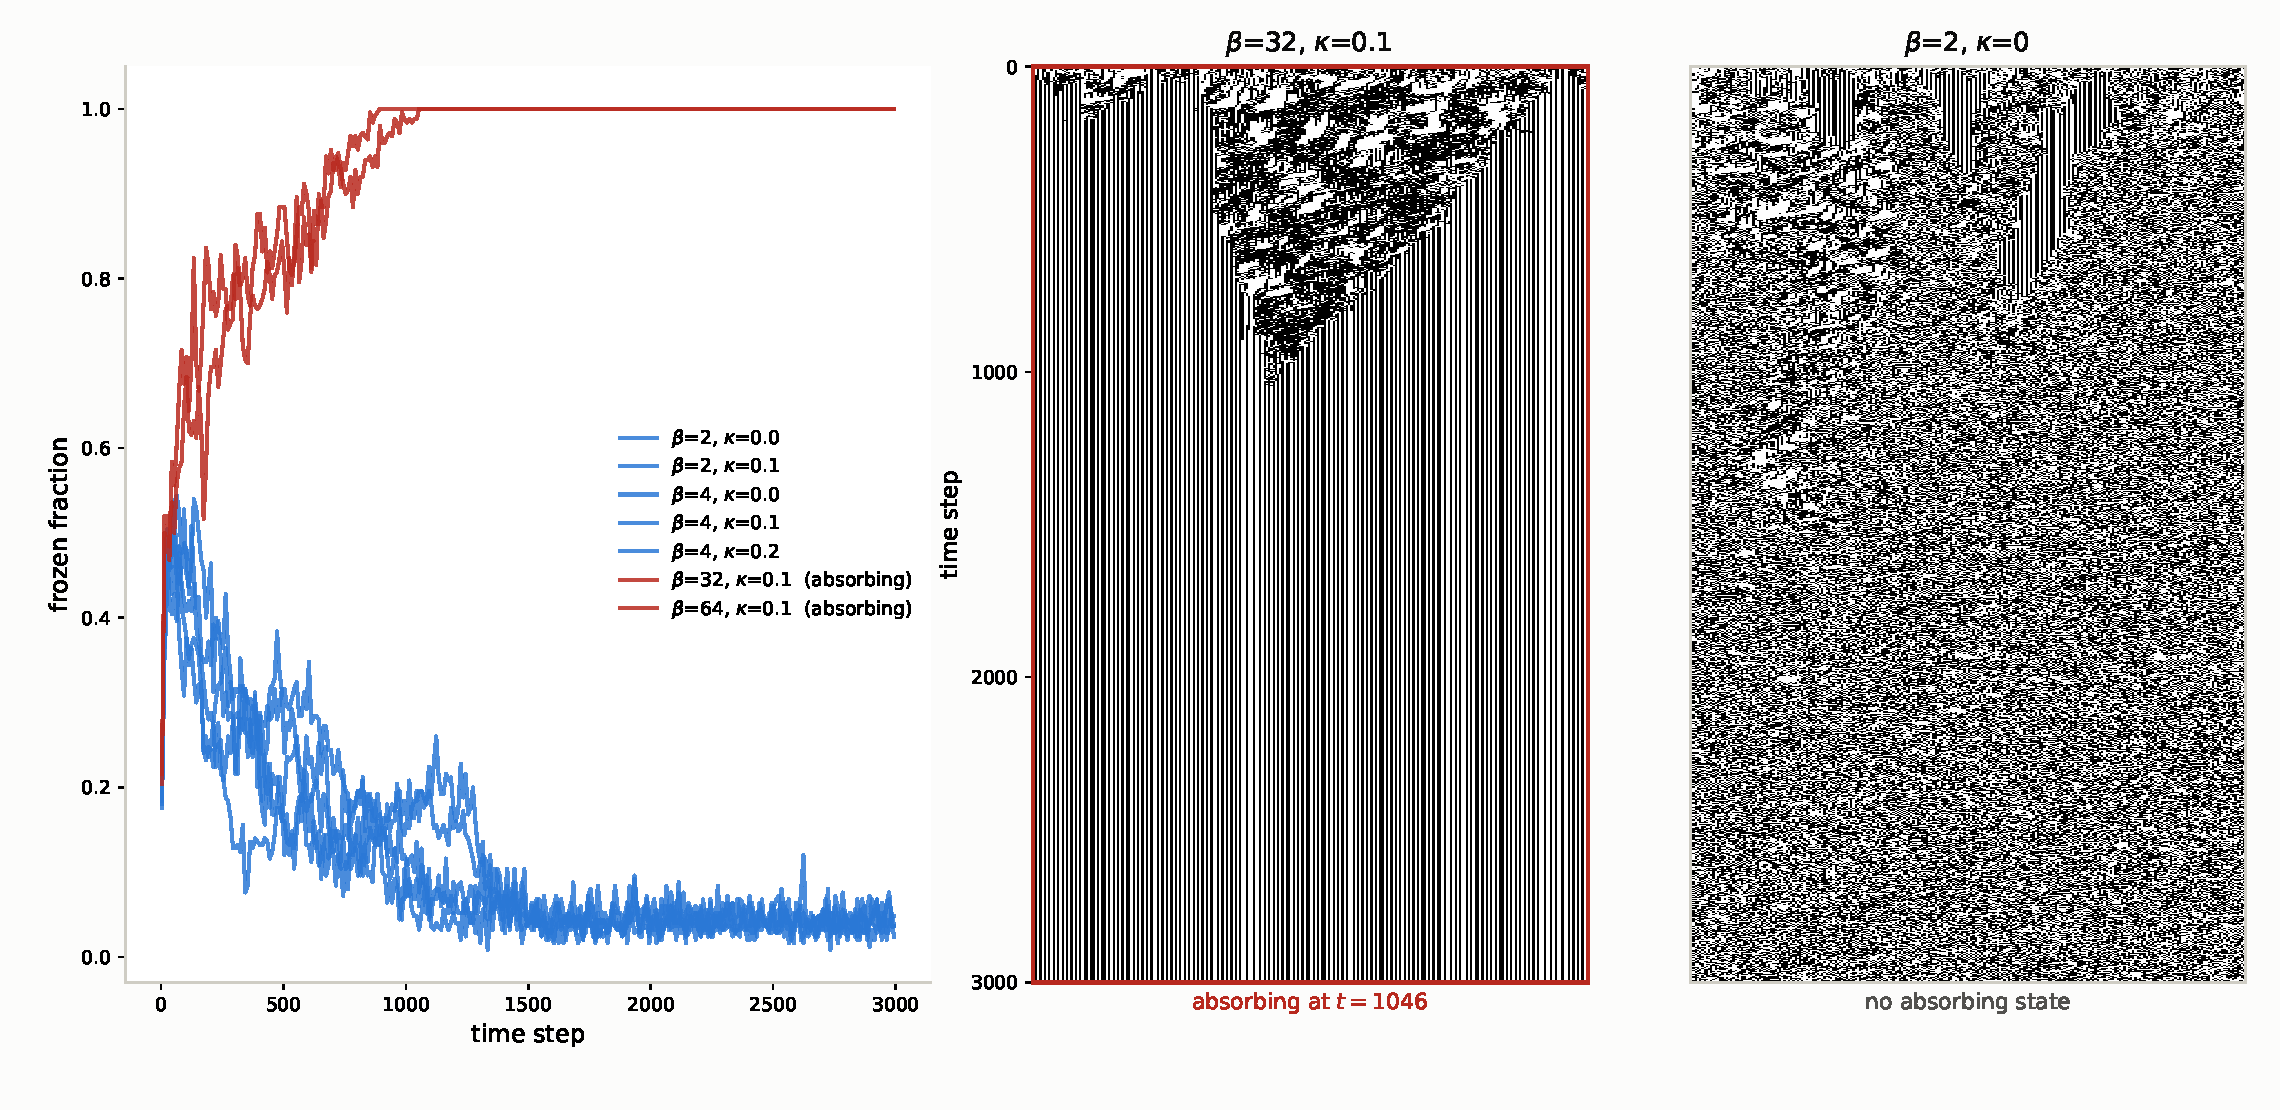
\includegraphics[width=\linewidth]{figures/exo-bifurcation.pdf}
\caption{The two arms of the ridge. Left: frozen fraction against time for the seven
configurations run to $3000$ steps, with the two that reach an absorbing state drawn in
red. The arms separate within the first few hundred steps and do not cross again. Centre
and right: the two extremes as spacetime diagrams --- $\beta = 32$, $\kappa = 0.1$, which
fragments the frozen field for some five hundred steps and is then squeezed out, against
$\beta = 2$, $\kappa = 0$, which erodes the frozen field to nothing and continues. The same
contest, opposite winners.}
\label{fig:exo-bifurcation}
\end{figure}

The two are the same kind of object---both carry coherent propagating
structure and sustained genotype diversity, differing in which phase
wins---and the search objective ranks them the wrong way round --- $0.625$ for the arm that dies against $0.422$
for the arm that lives. Across the seven configurations run to $3000$ steps on
two seeds the separation is perfect and inverted: every configuration that
reaches an absorbing state scored higher than every configuration that does not.

\subsection{At intermediate precision, both phases persist for ten thousand steps}

Between the two arms the objective falls to its minimum, and it is there that
the most interesting configuration sits. Bisecting $\beta$ between the arms at
$\kappa = 0.1$ locates the crossing between them: $\beta = 12$, $14$ and $16$ all
absorb, at $t = 1917$, $2604$ and $1722$; $\beta = 8$ and $\beta = 10$ do not.

At $\beta = 8$, $\kappa = 0.1$, one realisation sustains an intermediate state
for as long as we have run it. Across three windows spanning $10{,}000$ steps the
frozen fraction reads $0.071$, $0.048$ and $0.073$ --- neither collapsing to the
live-arm value of $0.04$ nor climbing toward one --- with $391$ distinct frozen
regions still forming and dissolving at $t = 9500$ and no absorbing state at any
point. The frozen phase is fine-grained and in continuous turnover: as spacetime
connected components the regions have a median lifetime of $24$ steps and a
median width of $4$ cells, and the largest reaches an area of only $650$, so
no region coarsens into a permanent continent within the observed horizon.

\begin{figure}[htbp]
\centering
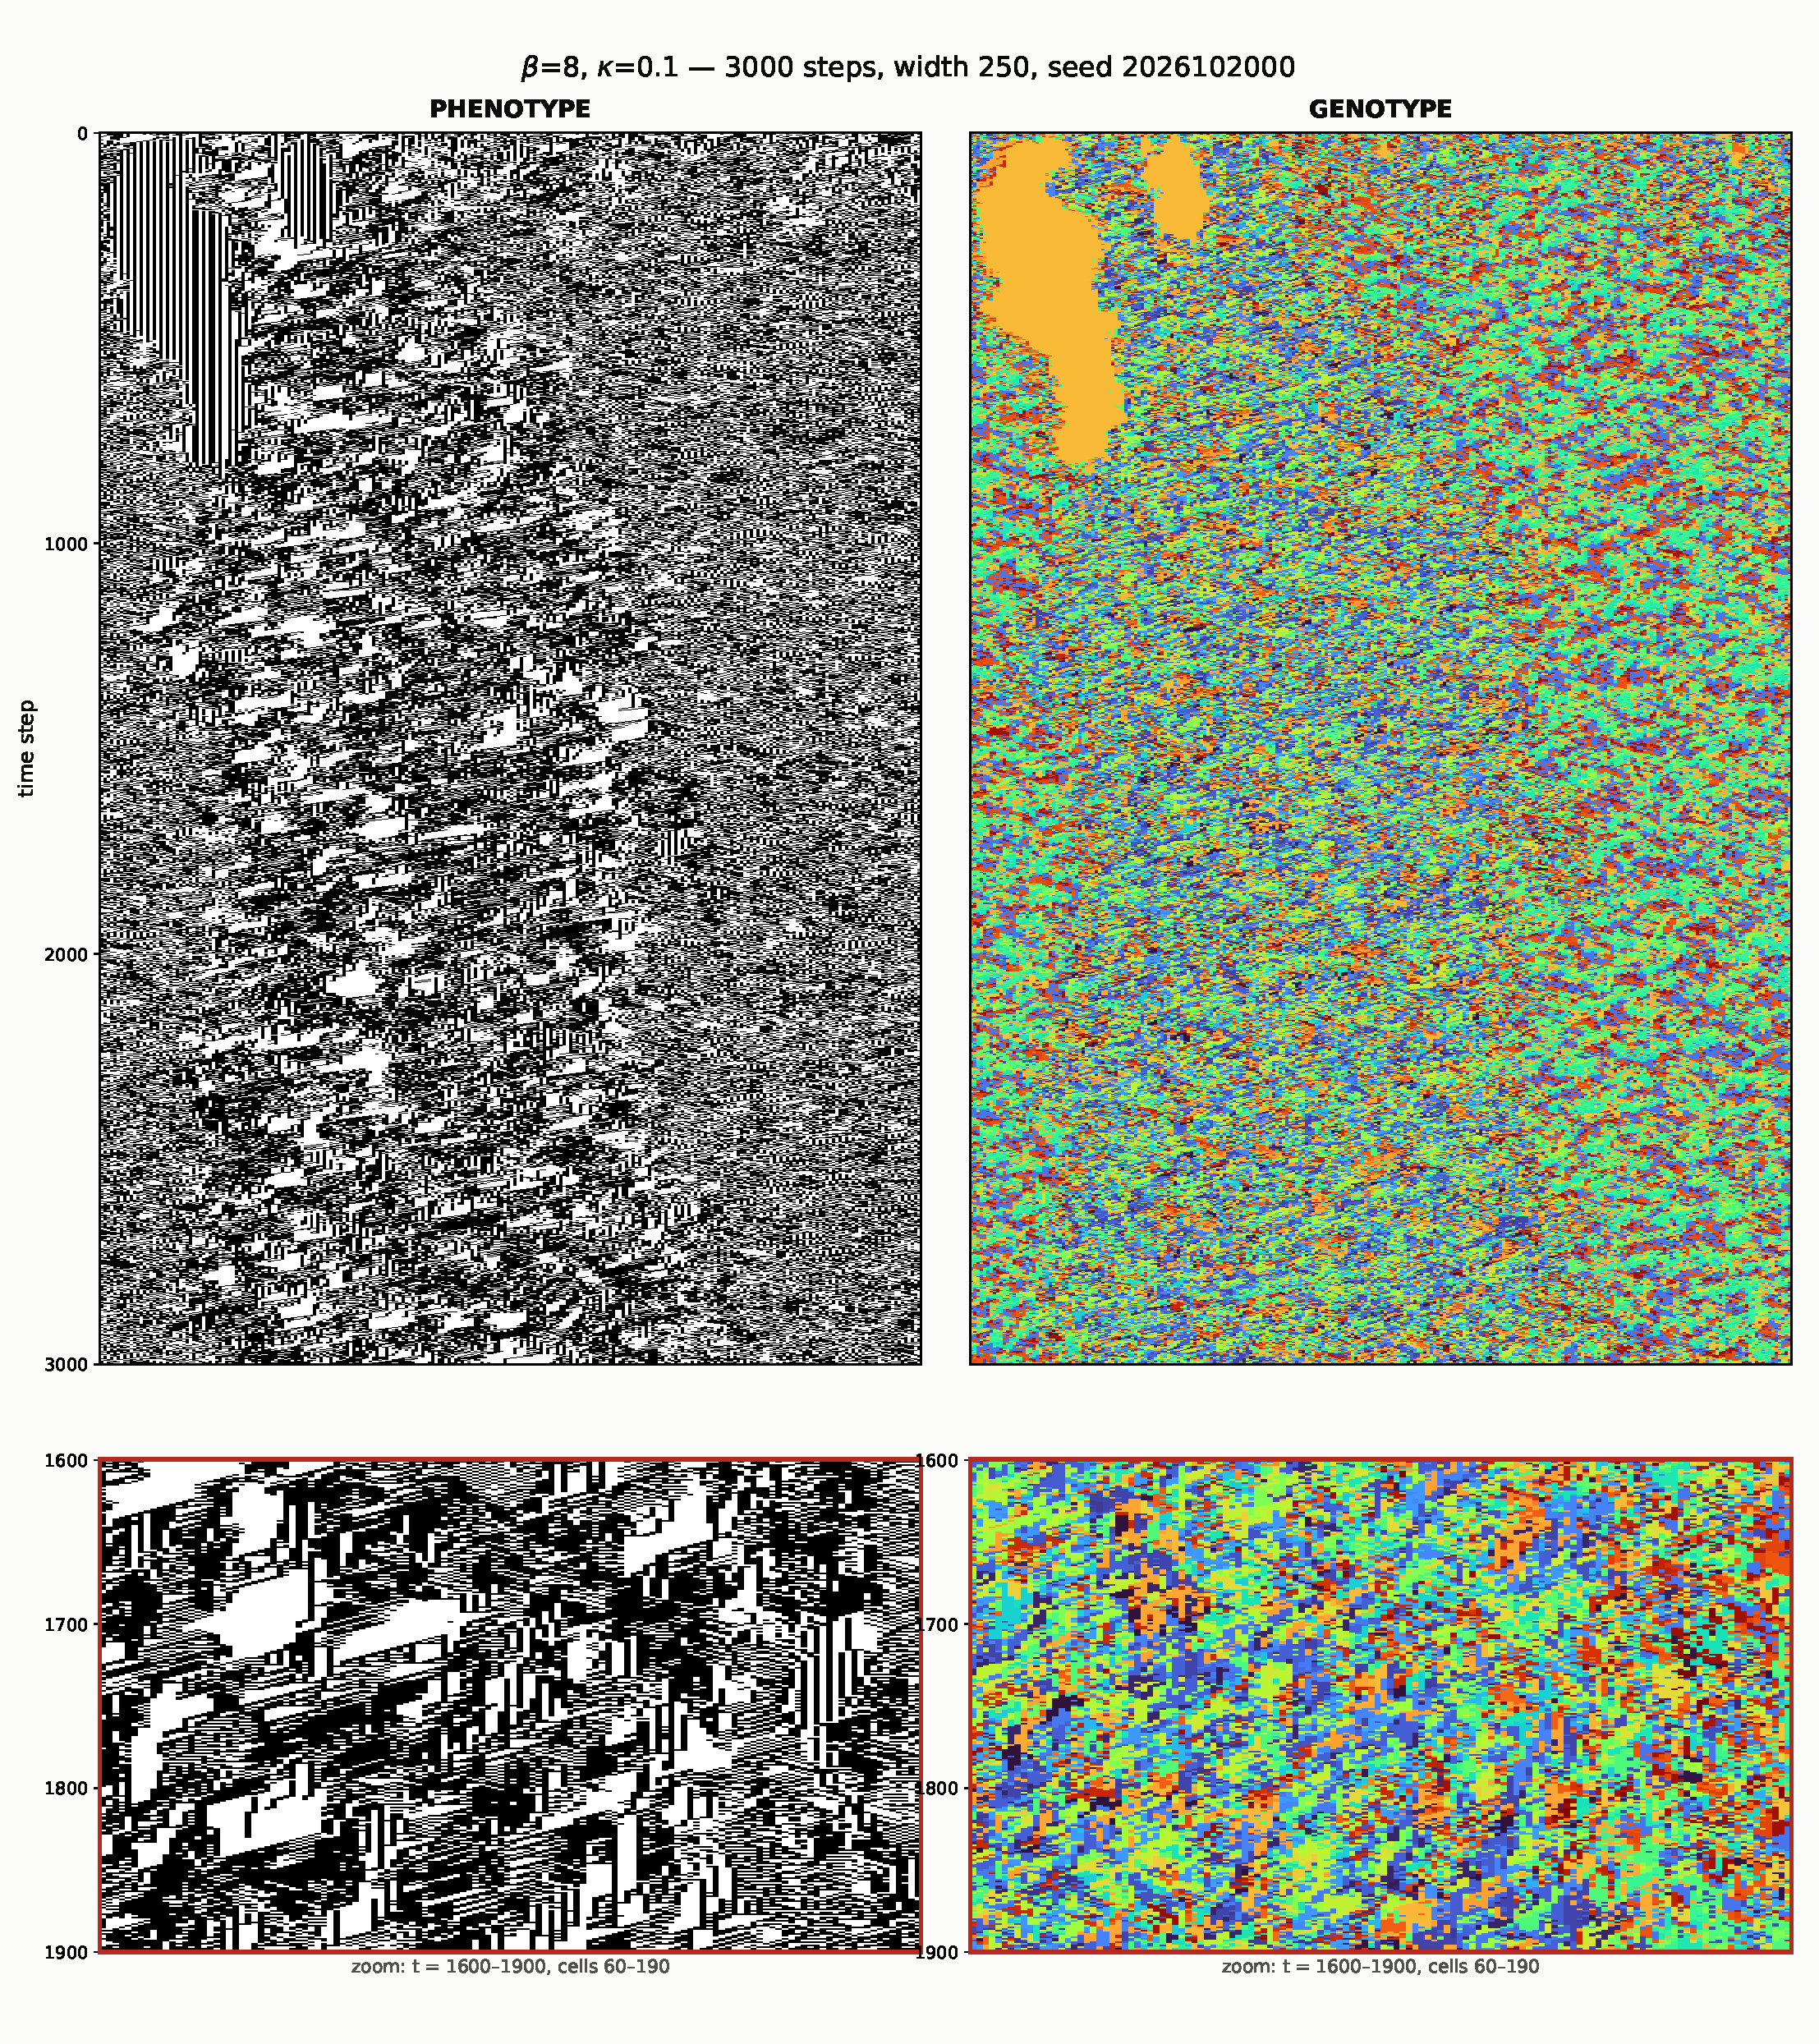
\includegraphics[width=\linewidth]{figures/exo-lavalamp-spacetime.pdf}
\caption{$\beta = 8$, $\kappa = 0.1$, both layers. Coherent diagonal propagating
structure runs the full sheet after the initial transient. The genotype carries
one monoculture region, gone by $t \approx 500$, and thereafter remains diverse
(mean row diversity $0.306$, churn $0.405$ per step, all $256$ sigils present).
The lower row zooms to the scale of the frozen regions, median $4$ cells by $24$
steps.}
\label{fig:exo-lavalamp}
\end{figure}

This configuration is the edge of chaos that the paper's opening example
first showed: frozen and moving structure coexisting, neither absorbing the
other---the thing such a search would have been built to find. It is also the one the objective ranks eighth of thirty-five, at
$0.453$, below both arms of its own ridge.

\subsection{The parameters do not determine which phase wins}

The honest description of this region is not that neither phase wins. It is that
\textbf{the parameters do not determine which phase wins.} The second seed at
$\beta = 8$ loses its frozen phase entirely, reading $0.103$, $0.000$ and
$0.001$ across the same three windows. At $\beta = 10$ the two seeds reach
\emph{opposite} outcomes: one sheds its frozen phase to $0.141$, the other
freezes completely and absorbs at $t = 6346$. Widening the lattice to $1000$
cells changes the answer again, and since that run also extended the horizon we
cannot attribute the change to width alone.

Realisation-to-realisation variance dominating a parameter's effect is what a
critical region looks like, and we report it as that rather than as a regime.
What the three examples establish is that this substrate contains configurations
of all three kinds --- one phase winning, the other winning, and neither winning
within the horizon we can afford --- and that they are separated by a bisectable
boundary in $\beta$. What they do not establish is a critical point, which would
require the intermediate behaviour to be a property of the parameters rather than
of the draw, and we have evidence against that at the two points tested.

\begin{figure}[htbp]
\centering
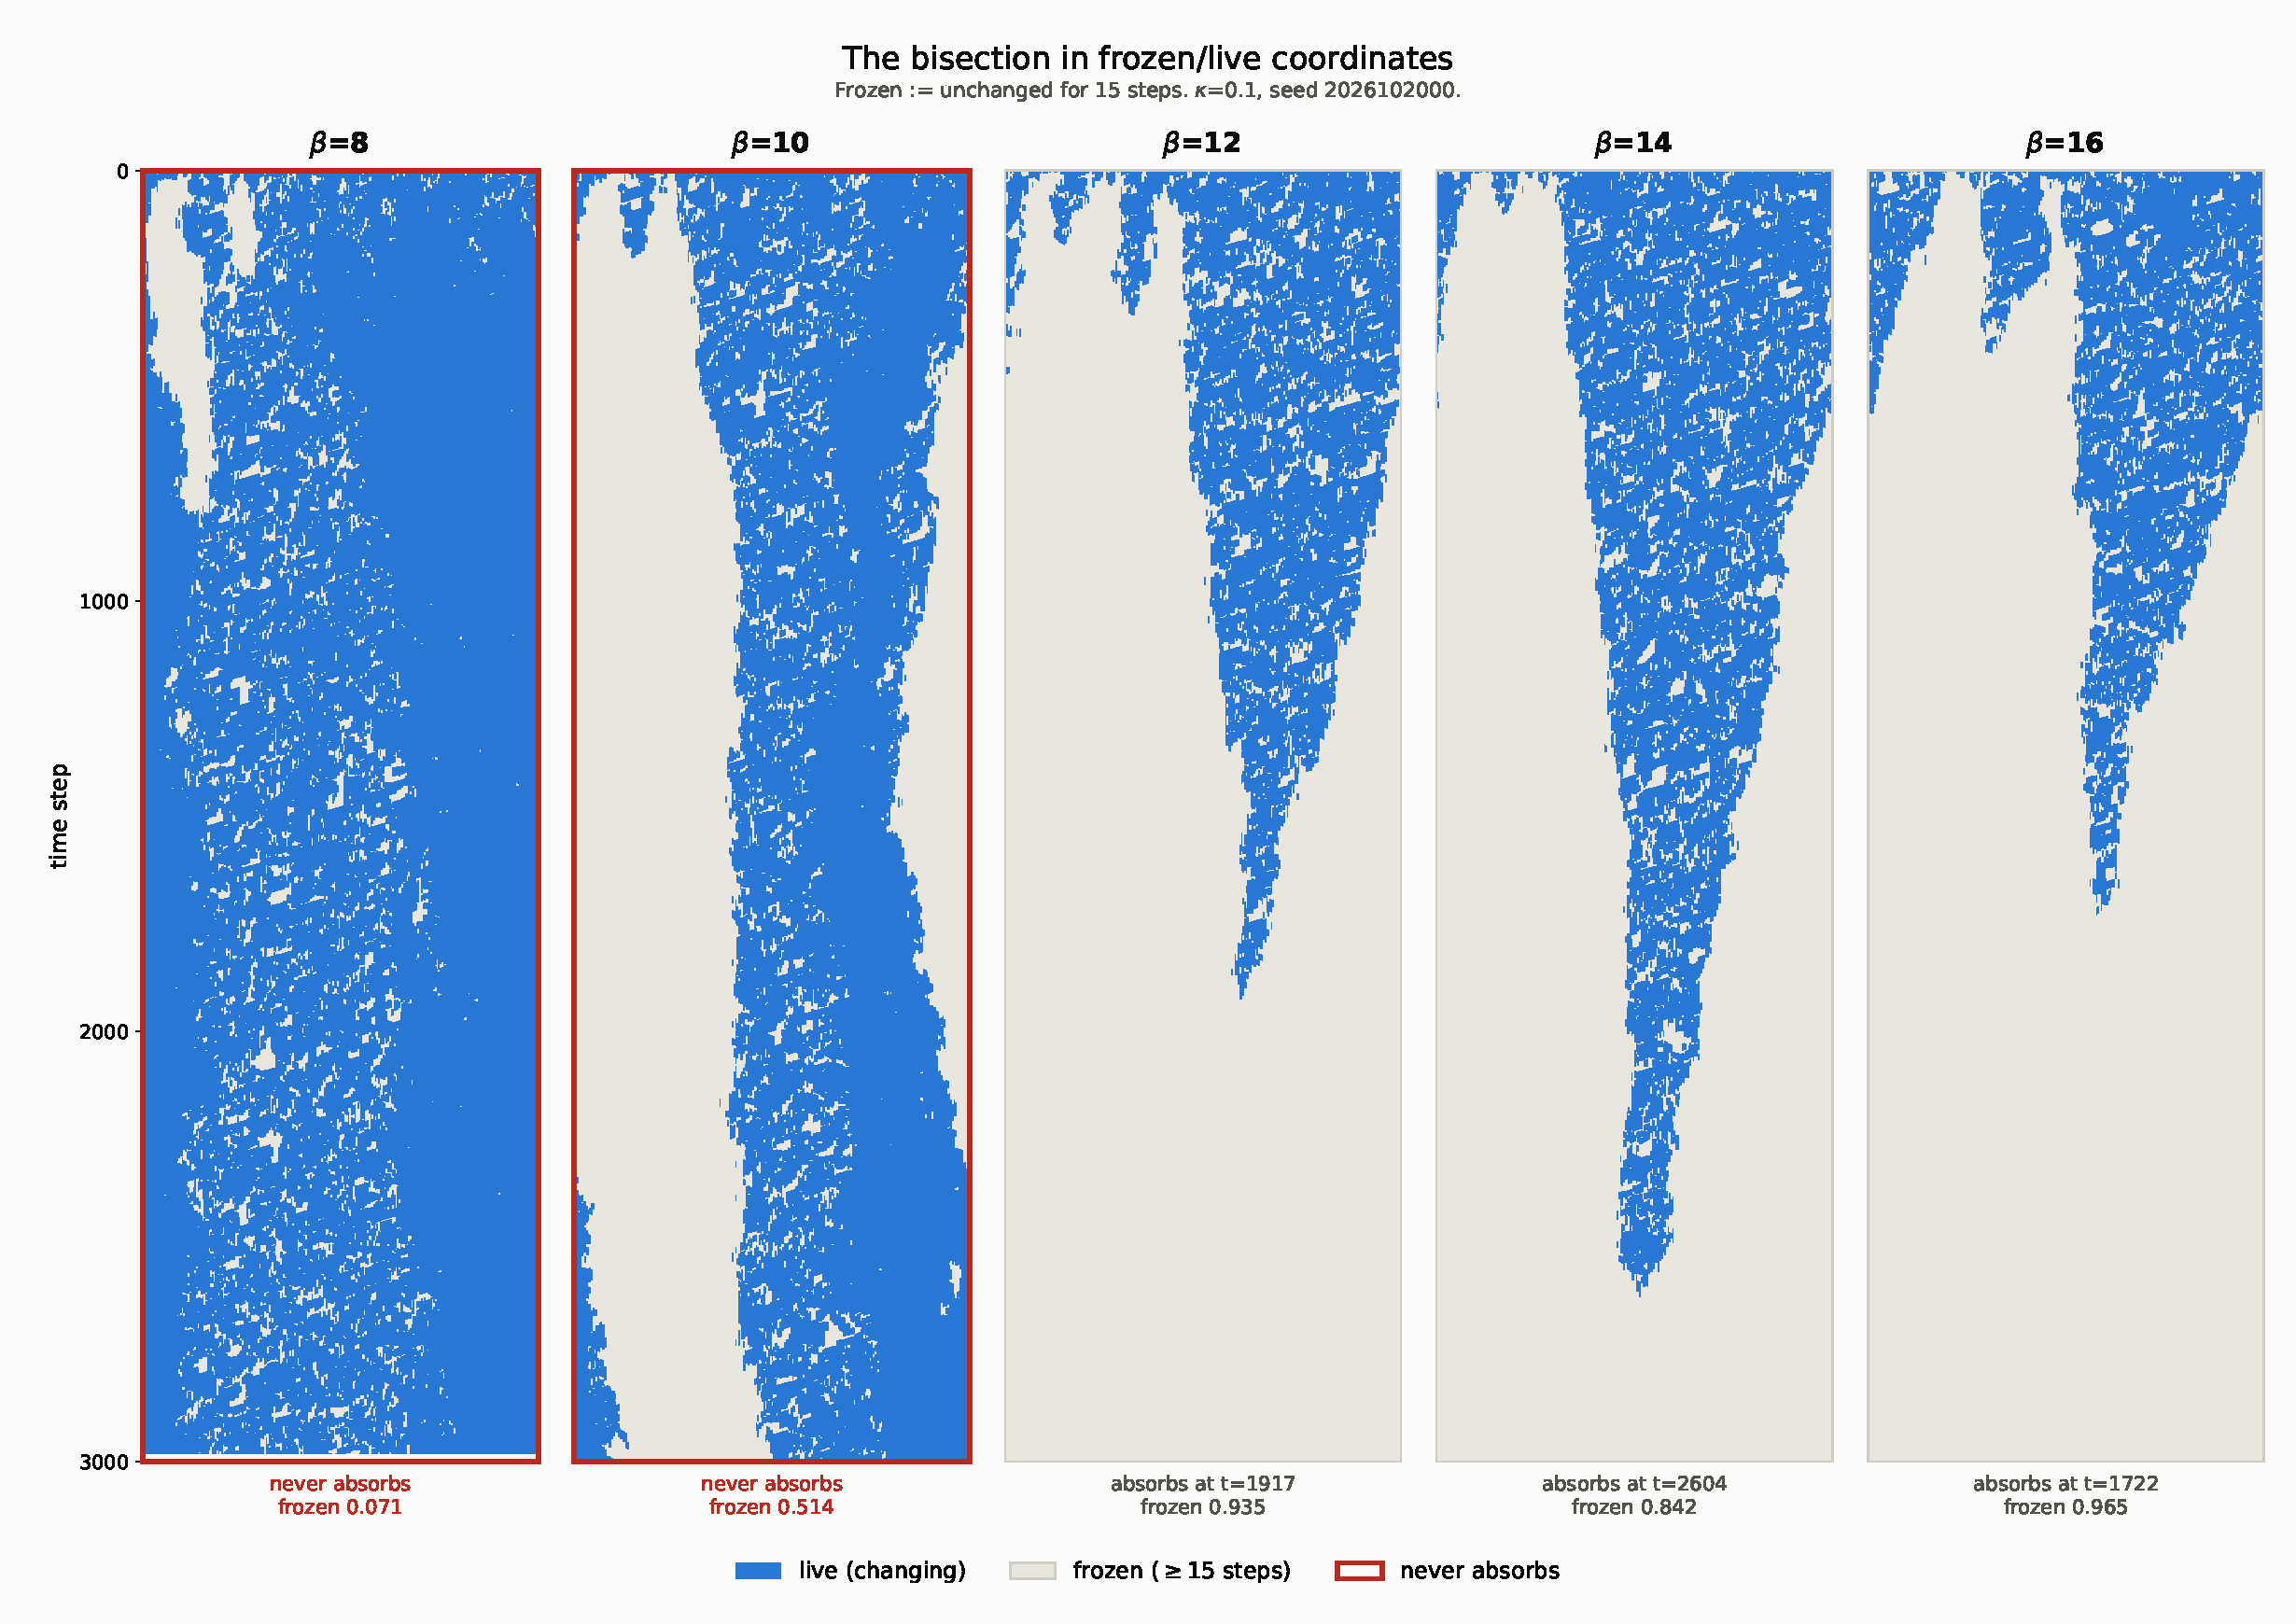
\includegraphics[width=\linewidth]{figures/exo-bisection.pdf}
\caption{The bisection in frozen/live coordinates, $\kappa = 0.1$. Frozen is
defined as unchanged for fifteen steps; at a four-step threshold the median
frozen episode is itself four steps and the turnover count inflates
thirteen-fold. $\beta = 12$, $14$ and $16$ taper to an absorbing state;
$\beta = 8$ and $10$ do not.}
\label{fig:exo-bisection}
\end{figure}

One methodological point generalises beyond these three examples and
dictates the section's use of persistence, rather than a short-window score,
as its measure. Every configuration reported here was present in the
thirty-five-configuration parameter sweep reported in Supplement~4 and was scored there over a $250$-step
window. At that horizon the example in the valley is unremarkable and the arm
that dies looks best. The behaviour that separates them --- absorption at
$t = 1046$, turnover sustained past $t = 9500$ --- occurs entirely outside the
window in which the objective was computed. An instrument validated on
$250$-step reference automata can be measuring a transient in a system whose
transients run four times longer.

\section{No Tested Local Quantity Finds Coexistence, and the Policy Creates the Absorbing States}
\label{sec:exotype-question}

Four deterministic measurements close the question posed in
\secref{sec:exotype-intro}. It separates into two parts---whether a cell can decide
from its own observations where the system should operate (search), and
whether a local rule can keep it there once placed (holding)---and both parts
close negatively.

\emph{The search half was external.} The search that located the examples
is described in Supplement~4: it swept a
thirty-five-cell grid over the selection rule's two parameters at four seeds
per cell, scored each run after the fact, moved over the resulting surface
under a learned surrogate, and restarted after every absorbed probe. None of
those operations is available to a cell inside a run, and the information
they produce arrives once per run rather than once per update decision. The
local substitute a within-run search would need---a cell ranking two
operators by a windowed observation of its own neighbourhood---fails at every
window length:
across eight seeds of the fixed-operator lattice the probability of a correct
pairwise ranking peaks at $0.571$ and \emph{decays} as the window grows, and
the comparison a cell can actually make, against its own neighbour, never
exceeds $0.540$.

The mechanism is a timescale mismatch. The frozen field---using the preceding section's definition, a site is frozen after fifteen unchanged phenotype steps---decorrelates at a site in about six steps, less than half the window
that gives the observable its discriminative power, so integration pools evidence
across contexts that no longer obtain---a fast decision fails by variance, a
slow one by staleness, and no decision rate exists at which feedback through a
temporally integrated detector works. The run-level result---that halting share and change rate predict local compressibility with held-out $R^2 = 0.73$---is unchanged; what fails is per-decision use.

\emph{The holding half is also negative within this family, with a reversal}
(Figure~\ref{fig:interventions}). The natural local mechanism---let cells that
sit in a pure neighbourhood, all frozen or all live, copy the operator of a
cell at a phase boundary, so that the mixed condition invades the pure---was
run at $\beta = 16$, $\kappa = 0.1$ the arm of the ridge that freezes solid.
It froze on all six seeds, and on five of the six \emph{earlier} than the
unmodified policy, by $297$ steps on average: at high precision the operators
found at boundaries are the freeze front's own, so boundary-directed copying
accelerates the phase it was built to resist. For the random-write intervention, each cell receives a fixed intervention interval sampled uniformly from 15 to 25 steps and a random phase offset; we call that interval its \emph{dwell}. When the interval elapses while the cell is in a pure neighbourhood, the cell receives one random operator write. This prevents absorption on all six seeds, but so does the same number of writes applied to uniformly random cells, to within seed noise, so the placement carries nothing. What either
preserves is a foam: small frozen islands, median width $2$ with the
majority at two cells or fewer, surrounded by changing sites, at a frozen
fraction near $0.3$ against the valley configuration's $0.08$ at the same
seed. Whether that state differs
from the valley configuration in \emph{structure} is not settled by the
statistics we computed: the coarse connected regions visible in
Figure~\ref{fig:exo-lavalamp} are a property of its spacetime components,
and under the per-step run-width statistic used here the valley runs measure
median $1$--$2$ as well. Undirected rule noise keeps this lattice alive; we
do not claim it keeps it at, or away from, the found configuration. A
complementary intervention targets the phase-boundary cells instead
(Figure~\ref{fig:interventions}, bottom row): at matched dose its outcome is
indistinguishable from its count-matched random-placement control, and at low dose it drives
the lattice to a near-frozen state threaded by one persistent changing seam
--- the write rate, not the placement, sets the outcome.

\begin{figure}[htbp]
\centering
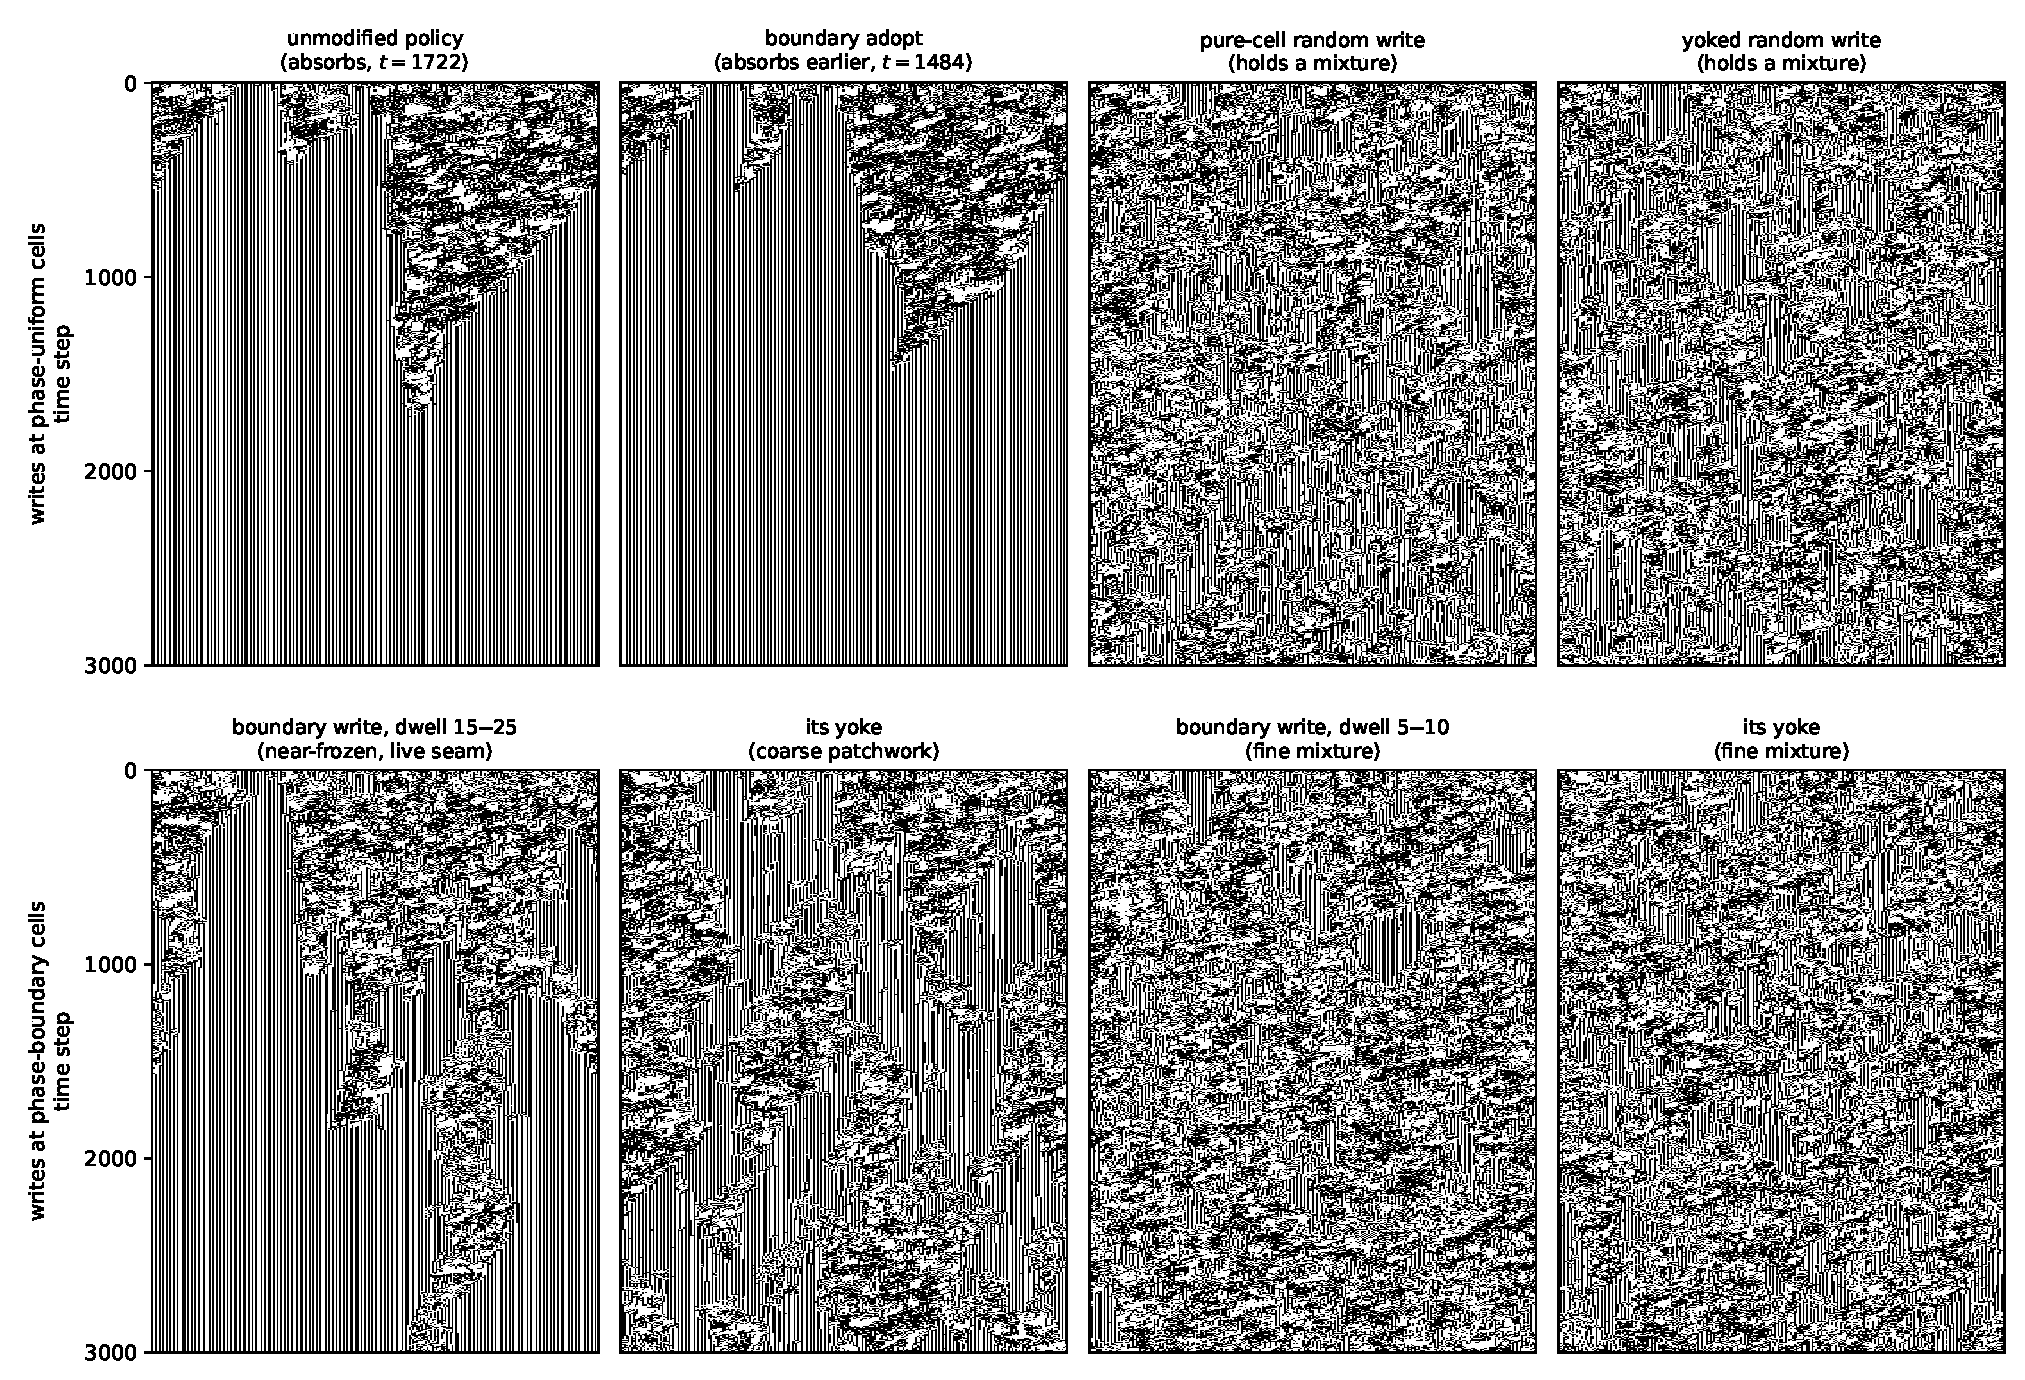
\includegraphics[width=\linewidth]{figures/interventions.pdf}
\caption{\textbf{Two local interventions at the freezing arm.} $\beta = 16$,
$\kappa = 0.1$, seed $2026102000$, whose unmodified-policy run is the absorbing $\beta=16$ example in Figure~\ref{fig:exo-bisection}; phenotype
spacetimes, all runs from identical initial conditions, frozen defined as
unchanged for fifteen steps. \emph{Top row}, writes at phase-uniform cells:
the unmodified selection policy absorbs at $t = 1722$; boundary-directed
adoption---cells in uniform surroundings copying the operator of a cell at a
phase boundary---absorbs \emph{earlier}, at $t = 1484$; one random operator
write per dwell at such cells prevents absorption, and so does the same
number of writes at uniformly random cells (median frozen-run width $2$,
frozen fraction near $0.3$ for both; across six seeds the pair is
statistically indistinguishable). \emph{Bottom row}, writes at
phase-boundary cells: at dwell $15$--$25$ the lattice approaches a frozen
state threaded by a persistent changing seam, while its count-matched yoke
holds a coarse patchwork; at dwell $5$--$10$ both arms hold a fine mixture.
Dose, not placement, sets the outcome at matched dose; at low dose the
boundary rule concentrates its writes on the remaining seam.}
\label{fig:interventions}
\end{figure}

\emph{A control changes what the question presupposes.} In the first no-adoption control, six runs use the same initial conditions as the six absorbing runs above, but the randomly assigned operators remain fixed; none freezes solid or dies out, and their frozen fractions remain between $0.083$ and $0.145$ through the full horizon. In a second no-adoption control at width $120$, all twenty-four runs likewise retain both changing and frozen sites, including runs begun from a deliberately frozen-leaning state. Within the tested
configuration family, then, freezing solid is an effect of the adoption rule
at high precision, not a behaviour of the lattice underneath: switch adoption
off and the same lattices, from the same starting points, hold a mixture
through the full horizon. The bisection that located the examples sits at a
different level entirely---it varied the rule's precision from outside,
between runs, and acted within none of them; it was a search tool, and this
control is what separates what it found from what the rule it varied does at
its extreme setting. Two boundaries on this statement matter.
First, its scope is thirty runs, two geometries, and one vocabulary of twelve operators; it is not a claim about rule-rewriting lattices generally.
Second, the uncontrolled state has not been shown to match the found
configuration in structure---the statistic that would separate or identify
them is not among those we computed. What the control establishes is
narrower: in this family, absorption is a property of running the selection
policy at high precision, not of the substrate the policy acts on.

\section{Two Probes from the Literature: the Freeze Is Nucleation-Limited, and a One-Sided Rule Holds a Mixture}
\label{sec:probes}

The related-work audit left two readings of Part~III open, and both are
directly testable. First, when a substrate co-evolves with the state on it,
a continuous absorbing transition classically becomes first order, with
bistability and hysteresis \parencite{gross2006epidemic}---a reading on
which the freezing of \secref{sec:exotype-question} is one branch of a bistable
pair rather than the endpoint of a crossover. Second, the one local design
class our interventions did not test is the asymmetric rule of
\textcite{droste2013analytical}: tentative while no information is
available, decisive on one-sided evidence.

The first reading is supported, in a specific form: the freeze is
\emph{nucleation-limited}. An adiabatic sweep of $\beta$ upward through the
freezing regime and back ($2{,}500$ steps per plateau, six seeds) produced
no freezing at any $\beta$ up to $32$ once the lattice had developed live
churn, and an extended dwell---$10{,}000$ steps at $\beta = 16$, six times
the cold-start absorption time---produced none either: transient settled
islands stayed below $3\%$ of the lattice and dissolved. Yet the same
dynamics from a cold start absorbs by $t \approx 1{,}700$ (the pipeline
reproduces \secref{sec:exotype-question}'s pinned-seed absorption to within one
step), and an \emph{established} frozen phase wins: a lattice spliced
half-and-half from an absorbed donor run and a churning donor run, restarted
at $\beta = 16$ with nothing done at the seam, was fully absorbed by the
frozen half in five of six seeds within $5{,}000$ steps. The frozen phase
invades any front it holds but cannot arise from churn at these horizons:
two macrostates persist at identical parameters, selected by the initial
condition, with a critical nucleus somewhere between the largest transient
island ($\sim$$7$ cells) and the spliced domain ($125$ cells). This is the
bistable phenomenology the co-evolving-substrate literature predicts, and it
scopes the crossover result of Part~I in the direction that literature
warns: at tested sizes, absence of a critical point and a
nucleation-limited first-order transition are not distinguishable.

The second reading is also confirmed, and it rescopes one sentence of
\secref{sec:exotype-question}. A cell whose phenotype has been unchanged for
$W^{*}$ steps is one-sided evidence of the frozen phase---live cells occur
in both macrostates and certify nothing. A rule that takes one random
vocabulary write at exactly such cells (refractory $15$ steps; nothing done
anywhere else) prevents absorption on all six seeds at $W^{*} = 100$ using
$0.51$ writes per step across the lattice; its count-matched control, the
same closed-loop write budget at uniformly random cells, needs $6.6$ times
the dose and still carries three times the frozen mass. Placement therefore
carries information once the trigger is one-sided; the earlier finding that
``the placement carries nothing'' is a fact about blind and cadence-triggered
writes, not about local intervention as such. The scope of the positive is
equally sharp: what the one-sided rule holds is a foam finer than the
noise arms' (median frozen-run width $1$; three-quarters of runs at two
cells or fewer; frozen fraction $0.17$), not the found configuration's
extended regions. The negative that stands is unchanged in kind but now
exactly bounded: no tested local quantity \emph{finds} the coexistence
condition, and no tested intervention---symmetric, blind, or
one-sided---recovers the \emph{found configuration}. What fell was only
the claim that local placement cannot matter.


\part*{Discussion}
\label{part:discussion}

\section{Limits}
\label{sec:limits}

The Part~I theorems are exact for the Boolean permutation core; its dynamical
claims are narrower and empirical. The census uses three seeds per operator,
the rotation survey two, and the finite-size scan $32$ per parameter cell, all
under the stated radius-one spatial protocol. These finite-run results do not
turn fixed-point balance into a claim about attraction. The substrate itself is
not new (\secref{sec:object}), and $\lambda$ is one heuristic among several
\parencite{wuensche1999classifying}; what is exact is only that the fixed-point
structure of Equation~\eqref{eq:prop} forces every fixed rule in the core to
have $\lambda=1/2$.

Part~II has different limits because it has a different object. Its central
causal comparison concerns one feedback-coupled construction rather than
either writing family, one lattice width, and six seeds. The descriptive
exponents are fitted over a range where damage width reaches only a tenth of
the lattice, so finite-size effects are not excluded. The architecture survey
and conservative-transport control compare mechanisms rather than exhaustively
sampling $8^8$ writings, and their fixed sample sizes are stated with each
result. They identify feedback and transport as controls in the tested
constructions, not as universal order parameters. The closing gate comparison uses one pair of constituents, one predicate
family, and sixteen seeds per row; a blind gate with matched correlation
length would separate current information from firing geometry, which the
present frozen control leaves entangled with a firing-fraction mismatch of up
to $0.04$. Illustrative diagrams use
pinned representative seeds. All reported computations are reproducible from
the accompanying package.

The Part~III results are bounded in three ways, each naming the experiment
that would extend it. \emph{Breadth}: the exotype
configurations sit at one arbitrarily placed point of the $40{,}320$-member
design space---twelve operators, selected neither to test a hypothesis nor to
cover the family, varied by no experiment; this is the most consequential
limitation of the work---with two seeds per parameter point---and those seeds disagree at two
points, so the region is reported without a critical point and with evidence
against one where tested; the closing measurements use six to eight seeds at
one geometry and one $\beta$. Varying $\sig$ along Part~I's classification
axes, and widening the seed sets, are the direct extensions.
\emph{Identified confounds}: the width-$1000$ persistence comparison changed
lattice width and duration together, so its outcome attributes to neither;
and the yoked
controls match override counts dynamically against their own lattice, so
realized doses can diverge between an arm and its yoke. Each names a control
that has not been run, not a flaw in one that has. \emph{Horizon}: all
persistence claims are bounded by the horizons actually run.

\section{Conclusion}
\label{sec:conclusion}

The paper has studied four related objects, and its conclusions must keep them
separate: permutation-propagators, update architectures, conditional compositions, and
per-cell exotype systems. Part~I concerns the finite permutation core. Its static results are
exact: a permutation-propagator possesses fixed rules exactly when all cycles
are even; an all-even permutation with $k$ cycles has $2^k$ fixed rules; and
every such rule is balanced, with $\lambda=1/2$. Its dynamical results are
finite-run observations over that core. The exhaustive census shows that all
odd-cycle operators remain genotype-alive under the stated protocol while
every all-even cycle type contains both sustaining and collapsing members. The
rotation survey and finite-size scan sharpen the distinction: fixed-point
existence does not determine attraction, and the tested propagator-fraction
scan gives a broad crossover rather than evidence of a critical point.

Part~II retains the two-layer lattice but changes the object from an individual
writing to an update architecture. The river construction composes a
permutation-propagator with a phenotype-reading step; the wider comparison adds
temporal schedules, mutation, holding, niches, and conservative local
transport. These are not a census of the $8^8$ writings, and the results do not
retroactively characterise the $8!$ core. They establish a narrower causal
claim. Against a matched feedback-off control, phenotype-to-genotype feedback
roughly doubles the reach of a single-cell perturbation. When the strength of
that feedback is varied, reach changes monotonically, while a control matched
in rule mobility but blind to the phenotype remains in the low-reach band.
Conservative transport further shows that sustained genotype diversity is not
itself the governing coordinate: high diversity can coexist with propagation,
and transport changes reach far more than diversity does.

The connection between the parts is argumentative rather than
theorem-to-theorem. Part~I proves that the classical $\lambda$ coordinate cannot
discriminate among fixed points in the permutation core and finds no critical
point in the tested parameter scan. Part~II asks what a causal measurement can
reveal once the architecture itself is allowed to change. Its answer is
feedback coupling for the constructions tested here, not a theorem about all
permutations or all writings.

This admits a reading the substrate makes unusually clean. The gain $\gamma$
interpolates between a genotype that reads only an ancestral phenotype and one
that reads the currently acquired state, with the frozen field a real phenotype
so that marginal statistics and spatial structure are matched at every setting;
only causal currency varies. What the dial varies is thus how legible acquired
state is to the heritable layer---the Lamarckian question, posed as a continuum
rather than a dichotomy. Its discriminating power is unusual in this family:
across $\lambda$, propagator fraction, sustained rule diversity, mutation rate,
refuge probability, niche width and rule mobility, causal reach stays below rule $90$'s
reference value, and blend strength alone passes it. The substrate carries no
fitness, so this concerns what the heritable layer can see and not what is
selected for. Part~II's closing gate measurements recover the same coordinate
from a construction sharing none of its dials---a blind condition reproduces
the dial, a phenotype-reading condition exceeds it, a frozen-phenotype
condition of matched width and firing rate does not---and that convergence is
the strongest connection the paper draws between its parts, though it is a
convergence of measurements rather than a theorem.

Part~III changes the object once more: the rewriting operator becomes state
the lattice carries per cell. Its measurements are persistence measurements
on single trajectories, and they close the question the part is organised
around: none of the local quantities tested locates the coexistence
condition, either to find it or to hold it---the
boundary-copying intervention accelerates the freezing it was built to
prevent---and within the tested configuration family, freezing solid occurs
only under the operator-adoption rule at high precision: the same lattices
with adoption switched off neither freeze nor die out.

The sample sizes, seed counts, and unresolved decompositions that bound each of
these claims are collected in \secref{sec:limits} and are not repeated here.

\paragraph{Future work.} Of the two extensions the gain result suggested, one is
in hand and one is transformed. An endogenous gain exists: a predicate reading
the lattice sets it, and reach responds to whether what the predicate reads is
current. A self-set operating point does not: two controllers failed for
reasons Supplement~4 records---one on leverage and stability, one because no
runtime-visible target survived validation---and the measurements of
\secref{sec:exotype-question} close the tested routes rather than only the attempts,
since in this substrate the local context decorrelates faster than any window
that discriminates. What replaces the search programme is a construction
question: the operator family contains members whose fixed rules form stable
media, and whether operating points can be \emph{laid out and held} rather than
found---structured regions of settled and active physics coexisting by
design---is open, cheap to test, and requires no cell to estimate anything.

The second extension is unchanged and remains the more interesting. As it stands the
substrate instantiates the Lamarckian arm alone: acquired state writes into the
heritable layer, and both the dial of Part~II and the gates of Part~III vary the
strength or the aim of that write-back. The Baldwin effect requires something this
substrate lacks---a selective filter, so that plasticity alters what selection sees and
the heritable layer follows without direct transcription. Adding selection over a
population of these architectures would supply that ingredient, and both arms could then
be compared externally on causal reach. We specified such an experiment before
building it, using the conditions of Supplement~4. Its first screen returned a negative
that reshaped the design rather than merely delaying it, and Supplement~4 reports what it
was and what it changed. A regulator operating from inside such a
population could not use that measure, for the reason Part~III gives, and would need a
persistence-like criterion instead; Supplement~4 sets out the conditions such an
experiment should satisfy before it is built.

\paragraph{Data and code availability.} Every numerical result in this paper is
regenerated from source rather than deposited: the generators are seeded, so a
single documented command rebuilds the fields underlying the tables, figures,
and reported summary statistics from an empty data directory, and the analysis
scripts consume no input that command does not produce. That command was run
twice from an empty data directory and all $307$ generated artefacts were
byte-identical across the two runs; the $298$ of them that also exist as
published artefacts match those as well. The closing measurements of
Part~III and the two figure panels added with them are generated by
standalone seeded scripts, named in the repository, that reproduce
deterministically but are not yet folded into that single command. The code and those
commands are publicly available at
\texttt{https://github.com/tothedarktowercame/mmca-clj} (commit
\texttt{7e04a6de6afe35de041b0ac4bb52a5cea25fe8d4})---a standalone,
dependency-light Clojure port of the MetaCA dynamics whose \texttt{README} gives
the complete reproduction command and commands for individual figure groups.
The classification and balance theorems are
formally verified in Lean~4 with Mathlib at
\texttt{https://github.com/tothedarktowercame/mathlib4}, branch \texttt{darktower}
(commit \texttt{bc34d8cec27216aae1d3cd511a9950ab1bce3575}), in
\texttt{DarkTower/Patterns/Propagator.lean}: the cycle-parity criterion as
\texttt{hasAlternatingColouring\_iff\_cycleType\_even} and the $\lambda = 1/2$
balance as \texttt{alternatingColouring\_true\_card\_eq\_four}. The same file
also contains executable regressions for both hand calculations, including the
displayed-position versus numerical-neighbourhood indexing contrast.

\paragraph{Generative-AI disclosure.} Anthropic Claude (Opus~4.8, Opus~5, and
Fable~5) and OpenAI Codex (version 5.6-sol) coding agents
\parencite{anthropic_claude,anthropic_fable,openai_codex} assisted in an
iterative, human-supervised workflow with manuscript editing, software
implementation, test construction, and adversarial checks. Exchanges with
Claude Fable~5 contributed to the initial identification of the operator family
reported here. The author reviewed the resulting prose and code, reran the
reported computations and formal checks, and accepts full responsibility for
the manuscript. Product information was accessed in July~2026; per-source
access dates are given in the bibliography.

\printbibliography
\end{document}
